\chapter{Hardware Architecture}

This chapter is devoted to the system's hardware architecture.
At first, the target hardware platforms will be introduced.
A strong emphasis will be given to the communication protocol and the interconnect architecture
as they were a pivotal point for this system's design.

Afterwards, the most significant system components will be presented.
There will be a discussion on their operation modes, 
the possible configurations, and the design trade-offs involved in their implementation.
We will present the final hardware designs that were implemented,
describing the reasoning behind the design choices.

The discussion will conclude with the application of partial reconfiguration technology
on this work. We will look into its physical aspects that affected our design,
the challenges of the floorplanning, and finally, the details of loading and configuring
a new accelerator.

\section{The Hardware Platform}

The primary hardware target of this work was the Zynq-7000 All Programmable SoC family from Xilinx.
An ``All Programmable SoC`` in Xilinx terminology or an ``SoC FPGA'' according to Altera/Intel and Microsemi,
is a device that combines a ``hard'' (i.e. implemented in silicon, not \gls{softip}) System-on-Chip
and the \gls{fabric} of an FPGA.

The notion of the ``SoC'' typically encompasses all the basic functional elements of
an embedded computer system capable to run a modern general purpose operating system,
excluding the main memory and storage. Still, vendors deviate from this definition --
Microsemi uses a microcontroller grade processing system based on Cortex-M3
which does not feature an MMU restricting operating system choice
\footnote{There is a port of GNU/Linux, the μClinux Project, that enables support of systems
that do not feature a Memory Management Unit. The port has been included in the mainline kernel.}
whereas Altera and Xilinx use the Cortex-A9 and A53 application processors. 
Still, the assortment of peripherals differ: 
Some devices omit even the GPU while others include secondary independent real-time processors.

The integrated FPGA \gls{fabric} is comparable that of the standalone FPGAs these vendors offer.
For example, the lower members of the Zynq-7000 family contain Artix-7 class \gls{fabric},
while the higher members contain a Kintex-7 class.

As a secondary hardware platform, a port for the Zynq UltraScale+ was made.
The port was intended to explore the significantly different (compared to Zynq 7000)
mechanics of partial reconfiguration 
as well as affirming the system's portability to a 64-bit SoC.

In the following table, the most important technical specifications 
of these two platforms are described.


\begin{figure}[ht!]
\centering
\resizebox{\textwidth}{!}{%
\begin{tabular}{cl cc}
\toprule
&			&Zynq 7000 & Zynq UltraScale+ \\
\cmidrule(l{.3em}r{.3em}){1-4}
\multirow{4}{*}{\rotatebox[origin=c]{90}{\small Board}}
&Development Board	& ZedBoard		& ZCU102 Evaluation Kit\\
&Device Model		& Z-7020 (-1)		& ZU9EG (-2)\\
&PS Memory		& 512MiB DDR3 (fixed)	& 4GiB ECC DDR4 SO-DIMM\\
&PL Memory		& n/a			& 512MiB DDR4 (fixed)\\
\cmidrule(l{.3em}r{.3em}){1-4}
\multirow{7}{*}{\rotatebox[origin=c]{90}{\small Processing System}}
&Main Processor		& ARM Cortex-A9 	& ARM Cortex-A53\\
&			& 32bit, 2 cores, 866MHz& 64bit, 4 cores, 1.5GHz\\
&			& L1 32kiB i/d per core	& 32kiB i/d per core\\
&			& L2 512KiB, OCM 256KiB	& L2 1024KiB, OCM 256kiB\\
&Real-Time Processor	& n/a			& ARM Cortex-R5\\
&			&			& 32bit, 2 cores, 600MHz\\
&Graphics Processor	& n/a			& Mali-400 MP2 667MHz\\
\cmidrule(l{.3em}r{.3em}){1-4}
\multirow{5}{*}{\rotatebox{90}{\small Programmable Logic}}
&FPGA fabric		& Artix-7 (28nm)	& UltraScale+ EG (16nm FinFET)\\
&LUT			& 53.2k 		& 274k	\\
&FF			& 106.4k		& 548k	\\
&BRAM (Mb)		& 4.9			& 32.1 \\
&DSP (slices)		& 220			& 2520 \\
&Transceivers		& n/a			& 24 GTH (16.3Gbps)\\
\bottomrule
\end{tabular}}
\caption{Technical specifications of the target hardware platforms.}
\label{tab:zynq}
\end{figure}

The internal interconnect of the Processing System (PS) and its 
connectivity with the Programmable Logic (PL) will be covered in detail in section \ref{sect:interconnect}.
Before that, it is important to describe the communication protocol
that all the on-chip interconnect utilizes.

\section{The Communication Protocol}

In order for two (or more) entities to exchange data, 
there must be a well-defined protocol.
With the growth of FPGA ecosystem, a need for a common 
and widespread communication protocol arose
in order to replace custom solutions that deemed 
too inflexible for bigger designs comprising IP
from different project teams and different companies.
The ARM's proposal is the \gls{amba}\cite{amba} protocol suite
which, as the name suggests, was initially deployed 
for microcontroller use but later expanded to SoCs
gaining momentum as a result of ARM's dominance in the smartphone market. 
Since all modern FPGA-SoCs from Xilinx use ARM cores, 
\gls{amba} became a natural choice for the company. 
Earlier products from Xilinx, like Virtex-II Pro which
featured a PowerPC core, used IBM's CoreConnect bus architecture. 
The other big contender is the free and open source ``Wishbone Protocol'', 
which, not unexpectedly, is the favorite of 
``OpenCores'' open-source hardware community.

The Zynq 7000 and the newer Zynq UltraScale+, 
the two platforms that are targeted by this work,
both feature ARM cores and are designed around the \gls{axi} protocol,
part of the \gls{amba} suite. 
As Xilinx tries to promote IP reuse with its IP Integrator tool,
it has expanded the use of \gls{axi} in its FPGAs that contain no ARM IP. 
The \gls{axi} infrastructure and several basic \gls{axi} peripherals
are offered by Xilinx in Vivado at no additional cost.
Therefore, \gls{axi} was chosen for the development of this system.

It is important to note that \gls{amba} protocols are for on-chip interconnect only.
Although they can transverse the PS-PL border,
they are never exposed outside of the chip. 
This stands true not only for Xilinx's -- or Altera's -- FPGAs, 
but also for all ARM-based microcontrollers and SoCs.

\subsection{The AMBA AXI Family}

\label{amba}
The \gls{axi} itself is essentially a group of protocols that support different topologies,
as well as feature levels that position themselves differently at the trade-off 
between performance and functionality versus silicon area.
However, they all share a fundamental bus concept: 
a multi-channel non shared-bus architecture that contains separate
channels for each \gls{transaction} type. It can be considered as a complementary
to \gls{ahb} protocol, also member of \gls{amba} suite, 
which is a single-channel multiple-master shared-bus architecture. 
Comparing these two families would give an edge to \gls{axi} in
throughput performance and clock frequency requirements, while \gls{ahb} would favor
better in terms of latency, wire count and power requirements. 
\emph{TODO: να βρω αξιόπιστη πηγή}

The \gls{axi} family has several members, but for this system the following three were used:
\begin{itemize}
\item	\textbf{\gls{axi}}, was the initial and only member in \gls{amba} 3.0. 
	With the advent of \gls{amba} 4.0 which introduced
	two new members described below, it is now usually 
	referred as ``Full \gls{axi}'' or ``\gls{axi} Memory Mapped''.
	The characterization of ``full'' contrasts to 
	the reduced capability \gls{axilite} and ``memory mapped''
	contrasts to \gls{axistream} which has no notion of address spaces.

	The \gls{axi} comprises five channels: Read Data (R), Read Address (AR),
	Write Data (W), Write Address (AW), Write Response (B). An \gls{axi} link
	may be unidirectional, discarding the unneeded channels.

	The addressing information must be communicated before a transfer to take place, 
	which consists a performance barrier. 
	To amend this, \gls{axi} supports \gls{burst} mode, 
	where sequential \glspl{beat} of data may be transferred without 
	re-transmitting any addressing information.
	Between the two communicating endpoints, 
	an intermediary ``\gls{axi} Interconnect'' must be inserted.

	Its typical use in the FPGA realm is transferring data between memory resources,
 	like \glspl{bram}, processor RAM, FPGA memory controllers, etc.

\item	\textbf{\gls{axilite}}. Introduced with \gls{amba} 4.0, 
	the \gls{axilite}, as the  name implies,
	is a reduced capability version of \gls{axi}. 
	The most notable simplification is the 
	lack of support for \gls{burst} transfers. 
	In exchange, it offers a much lower silicon footprint. 
	
	It is best suited for low intensity traffic, 
	typically for configuration or status registers.

\item	\textbf{\gls{axistream}}. Also introduced with \gls{amba} 4.0, 
	\gls{axi}-Stream is a data streaming protocol,
	which means that it has no notion of memory addressing.
	This greatly simplifies implementation and reduces wire count.
	Data flows from the one endpoint to the other, in one direction, 
	without the need of any intermediary interconnect.
	Transmission size is not known in advance; data will flow
	indefinitely until a control signal (TLAST) is asserted.

	\gls{axistream} allows the addition of user defined out-of-band data,
	typically for synchronization, and it supports sender and receiver IDs, 
	which enables stream routing for virtual circuits.
\end{itemize}

None of these protocols supports cache coherency. 
In \gls{amba} 3.0, ARM proposed the \gls{acp}, 
an \gls{axi} slave port that connects an \gls{axi} master directly to the processor.
The coherency logic inside the processor 
will monitor the transactions and update its caches accordingly.
However, since the \gls{axi} master is not aware of the cache coherency logic, 
\gls{acp} is only an \gls{IO Coherency} mechanism;
the processor caches may be coherent but the accelerator's are not.

In \gls{amba} 4.0, ARM extended the \gls{axi} protocol with \gls{ace}, 
which allows full coherency between the processor and the accelerator, 
and \gls{acelite}, an \glslink{IO Coherency}{IO Coherent} version.
The latter differs from \gls{acp} in that its coherency is managed
by the interconnect and therefore the port requires no proximity
to the processor. 
These protocols are supported in the newer UltraScale+ but not in the Zynq-7000.

Finally, in latest \gls{amba} version, 5.0, ARM added \gls{chi}, 
which targets the multiprocessor's local interconnect hub.

In the data streaming model that this work targets, 
there exists no spatial or temporal locality. 
Cached transfers are not only useless but harmful, 
since they will cause cache thrashing. 

Indeed, the kernel driver uses the Linux DMA Streaming API
which bypasses all processor caches by marking 
the allocated DMA'able pages as non-cacheable.
Therefore, cache coherency will not matter our discussion any further;
however, the hardware interconnect that implements these cache-coherent
protocols may be of our use and therefore it will be examined.

\subsection{The AXI Implementation}

The \gls{axi} implementation in Xilinx products consists of the hardware 
implementation in Zynq 7000 and Zynq UltraScale+ devices,
the \gls{softip} protocol infrastructure offered in IP Integrator, 
and the \gls{axi} compatible IP building blocks. 
Additionally, Xilinx offers automation for creating 
custom cores with \gls{axi} interfaces.
It is worth to cover this functionality as 
part of understanding the connectivity of the system.

\subsubsection{The Zynq Hard IP}

The Zynq 7000 is built around \gls{amba} 3.0. 
The interconnect will be presented at the next section,
but it is important to mention here that 
the use of \gls{axi} of this \gls{amba} version
carries two important restrictions: 
The original specification of \gls{axi},
as is present in \gls{amba} 3.0 has a maximum \gls{burst} size of 16. 
Any \gls{axi} master residing in PL that connects to the PS through a slave port,
will have to obey this limit or use a protocol converter.
Secondly, \gls{amba} 3.0 does not support \gls{axilite} or \gls{axistream}, 
therefore all ports in Zynq-7000 are Full \gls{axi}.

The Zynq UltraScale+ is \gls{amba} 4.0 compliant. 
Therefore, both of the aforementioned issues do not apply.
Still, the \gls{afi} that supports the \glsdisp{hp}{HP} ports is version 3 only,
and protocol conversion takes place in silicon. 
This process in transparent to the designer but is still important
as it affects performance.

\subsubsection{The Xilinx Soft IP}
\label{sect:xilinx-ip}

At the PL front, Xilinx offers a suite of 
IP cores that manipulate the \gls{axi} traffic.
It offers cores for conversion (stream combining, 
width conversion), buffering (clock conversion,
stream pipelining, \gls{fifo} buffers) and routing 
(stream broadcasting, stream switching, \gls{axi} crossbar).
Additionally there are some higher level \gls{axi} building blocks
that automate the interconnect of \gls{axi} endpoints. 
Due to their importance, it is worth to be mentioned separately:

\begin{itemize}
\item	\textbf{AXI Interconnect}.
	It can connect $M$ \gls{axi} masters to \gls{axi} $N$ slaves 
	communicating with either the Full \gls{axi},
	both version 3.0 and 4.0, or the \gls{axilite} protocol.
	The interconnect can be configured in full crossbar mode 
	(shared address, multiple data) for high performance,
	or in shared access mode (shared address, shared data) 
	for low area use, issuing only one transaction at a time.
	
	The AXI Interconnect is build around the AXI Crossbar. 
	The AXI Crossbar implements the core switching functionality 
	and the AXI Interconnect wraps it with the appropriate port couplers that may
	perform necessary clock and width conversion and/or append register slices or FIFO buffers,
	to help timing closure and smooth traffic, respectively.

	The AXI Crossbar allows the definition of a connectivity matrix 
	for sparse crossbar implementation. 
	However this feature is not used by AXI Interconnect and if desired,
	the designer must instantiate the AXI Crossbar and its couplers manually.

\item	\textbf{AXI SmartConnect}. 
	This core is a newer design with functionality analogous to \gls{axi} Interconnect.
	It is advertised to be highly optimized to mitigate wire delays in UltraScale+.
	However that comes at some cost in FPGA resources.
	If the design uses a slow clock for the targeted FPGA or 
	if the slaves are \gls{axilite} configuration registers,
	the older \gls{axi} Interconnect should be preferred.

\item	\textbf{AXI Stream Interconnect}. 
	The equivalent interconnect for \gls{axistream}, 
	as it can interface $M$ \gls{axi}-Stream masters to $N$ slaves.
	Likewise its sibling, it is built around the AXI-Stream Switch with the appropriate
	couplers in each of its interfaces.

	The stream routing may either be defined externally through 
	a configuration register or by sender / receiver IDs. 
	It should be stressed that in contrast to its Full \gls{axi} counterparts, 
	it is not an essential core if only a single master is connected to a single slave.
	Its use arises on shared physical links and/or where virtual circuit switching is needed.
\end{itemize}

Xilinx offers a few DMA controllers, compatible with both the full AXI and the AXI Stream.
If implemented in the programmable logic, they can move data between an
addressable memory resource and either another one, or alternatively stream it
to a memoryless component. These are the solutions offered:

\begin{itemize}

\item	\textbf{AXI DataMover}:
	This is the central component of all DMA controllers.
	Its role is to move data between the memory mapped and the streaming domain.
	It needs external logic for control, a role that is assumed
	by the three DMA controllers described below.
\item	\textbf{AXI DMA}:
	The AXI DMA can generate \gls{axistream} compatible streams
	from a full \gls{axi} compatible addressable memory resource.
	Its core are two unidirectional or a single bidirectional
	\footnote{This configuration is not supported by Xilinx HSI for DeviceTree generation,
	which is the standard method describing hardware to the Linux kernel}
	AXI DataMover.
	It is configured by an \gls{axilite} interface.
	The core has an optional scatter-gather engine that can continuously fetch and execute
	transfer descriptors without any pause as well as optional multichannel support.

\item	\textbf{AXI Video DMA}: 
	This core is a variation of the AXI DMA specialized in video streams.
	Among other optimizations, it takes advantage of the user-defined out-of-band channel
	of \gls{axistream} for frame synchronization.

\item	\textbf{Central DMA}: 
	The Central DMA, probably a misnomer, can move data between two Full \gls{axi}
	compatible slaves, e.g. the processor memory and an \gls{axi} BRAM controller.
	It is implemented by a bidirectional DataMover and the control logic, with an optional
	scatter-gather engine. 
 \end{itemize}


\subsubsection{The User IP}

As it becomes clear, Xilinx does offer a significant amount of 
\gls{axi} infrastructure IP and \gls{axi} compatible peripherals
to support the implementation of an \gls{axi}-based system.
Still, implementation of \gls{axi} compliant custom logic is a non-trivial task to undertake.
Depending on the workflow and the designer's experience and demands,
there are five options available.

\begin{itemize}
\item	\textbf{Custom Implementation}:
	In case that maximum flexibility and performance is desired,
	a custom implementation is the way to go. 
	Xilinx offers an \gls{axi} Verification IP 
	which helps the designer to verify the functionality of an RTL design.

\item	\textbf{IP Integrator}:
	Xilinx offers a ``Create and Package IP'' wizard in its IP Integrator tool.
	The designer may define the desired \gls{axi} parameters 
	and the wizard will generate the corresponding RTL code
	to create the \gls{axi} interface. 
	The designer can afterwards tweak the code to adapt their needs.

\item	\textbf{IP Interfaces (IPIFs)}:
	IPIFs are IP cores that alleviate the burden of \gls{axi} conformance 
	from the end designer by performing the complex \gls{axi} signaling 
	themselves while offering a simple memory-like interface on the other end. 
	Xilinx provides two such cores, one for Full \gls{axi} 
	supporting \gls{burst} transactions, and one for \gls{axilite}.

\item	\textbf{Bridges}: In case the user IP is already developed with an alternative protocol,
	it may be possible to be bridged to the \gls{axi} interconnect, 
	if the additional overhead can be tolerated.
	Xilinx provides only a handful of bridges, mostly of use within the \gls{amba} family, 
	e.g. for \gls{ahblite} (both slaves and masters) and for \gls{apb} (slaves only). 
	However, additional bridges may be found at OpenCores or in other open-source libraries. 
	In the simplest case possible, a designer may even opt for 
	the \gls{axi} \gls{gpio} core that can provide up to two 32 bit general purpose I/O lines.

\item	\textbf{HLS}: If the designer uses the Vivado High-Level Synthesis workflow,
	the tool is able generate \gls{axi} compliant IP using simple HLS directives. 
	This is particularly useful to implement the HLS-core control protocol over \gls{axilite}.
\end{itemize}

\section{The Physical Interconnect}
\label{sect:interconnect}

So far, we discussed the communication protocol and its implementation at both 
the programmable logic and the silicon domains.
The next logical step would be to examine the underlying physical interconnect
that supports it on the SoC-FPGAs that this work targets. 

Granted, in the FPGA \gls{fabric} there is infinite flexibility and any topology may be created.
The presence of a hard IP however, presents a constraining factor.
In both Zynq 7000 and UltraScale+ series, 
there is a single multi-port memory controller
that resides on the PS side. Therefore, any traffic from/to the PL must
first cross the PL-PS boundary, then be routed inside the PS interconnect,
and finally reach a memory controller port. 

Understanding the nature of this path is not a trivial matter. 
Nonetheless, it imposes a number of hardware and software decisions
in this work's implementation, and therefore it needs to be analyzed.

Since the architectural details of these two SoC-FPGA families are
significantly different, they will be covered separately.

\subsection{The Zynq 7000 Interconnect Architecture}

The 7000 series glues the PL and PS together with a number of
high speed ports of varying functionality. Most are slave ports to the
PL, which means the transaction initiator must reside in the programmable logic.
A couple of them are master ports, to be driven by either the ARM cores,
the PS DMA controller or some I/O peripheral. 
One of them is able to provide \gls{IO Coherency},
but there is no support for two-way, full coherency.

The figure \ref{fig:zynq7000-interconnect} presents the system architecture 
of Zynq 7000 series, emphasizing the interconnect. 
Technical details are sourced from \cite{ug585}.

\begin{figure}[htbp]
  \centering
  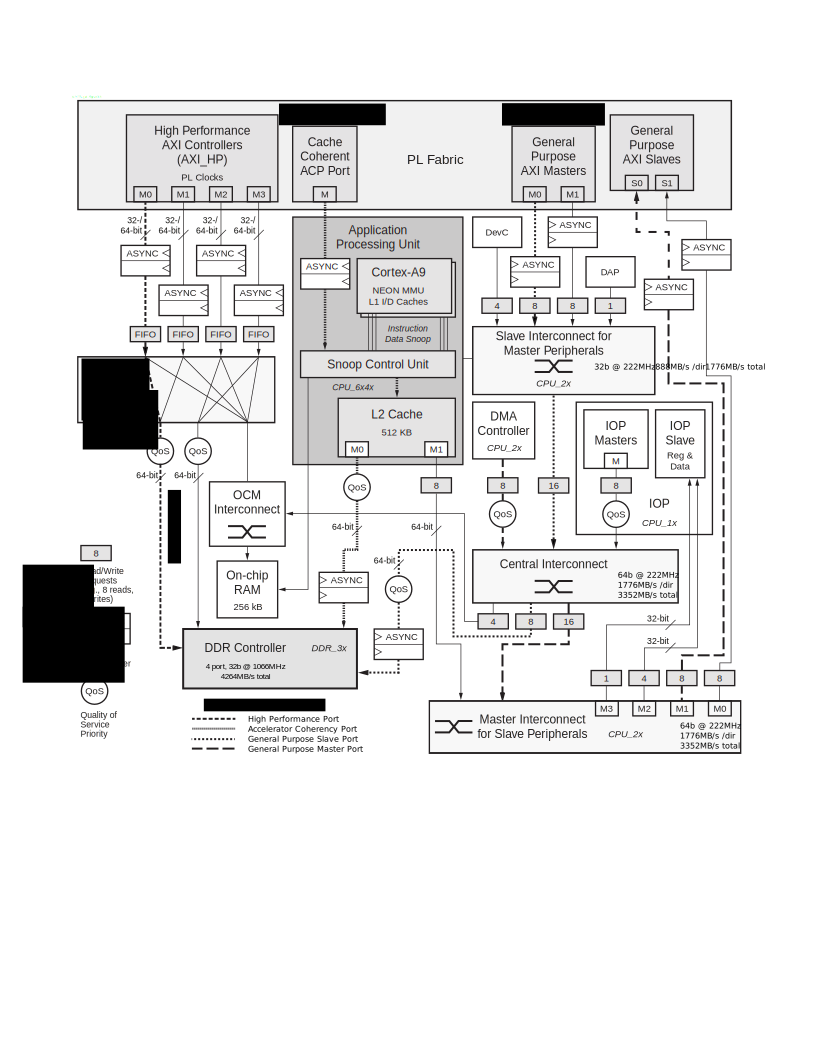
\includegraphics[scale=.9,center,trim={0 75mm 0 0},clip]{img/zynq-7000.pdf}
  \caption{The Zynq 7000 system architecture. 
  Note that port naming follows the controller role, not the port's.
  For example, the ``GP \gls{axi} Masters'' are connected to the
  ``GP \gls{axi} Slave Ports'', titled ``M0'' and ``M1''. Conversely,
  the ``GP \gls{axi} Slaves'' are connected to the ``GP \gls{axi} Master Ports'', titled ``S0'' and ``S1''.
  Modified image from \cite{ug585}.
  }
  \label{fig:zynq7000-interconnect}
\end{figure}

\subsubsection{The High Performance Ports}
\label{sect:zynq7000-hp}

The Zynq 7000 provides four \gls{hp} ports, HP0 to HP3.
These are all slave ports to the PL, conforming to \gls{axi} version 3.
If the \gls{axi} master is implemented in \gls{axi}4, as is the usual case,
protocol conversion must take place in the PL.

The ports are clocked by a PL clock at up to 150MHz, and can be 32 or 64 bit wide.
As the \gls{axi} protocol mandates, they have separate wires for each direction,
offering a per direction bandwidth of 1200MB/s for each port.

The \gls{hp} ports are connected to the memory controller through the Memory Interconnect
which in turn drives two of the four ports of the memory controllers, as well as
one port of the \gls{ocm} interconnect.
The port clock will be converted to 355MHz,
offering a switching speed of 2840MB/s per direction, 5680MB/s total.
The switching scheme routes the traffic from the first two \gls{hp} ports 
to the first memory port, and the other two \gls{hp} ports to the second. 
Any port can be routed to the \gls{ocm}.

The memory controller offers an aggregate bandwidth of 4264MB/s 
shared among its four ports, irrespectively of the data flow direction.
Therefore, if all \gls{hp} ports are used and configured at their maximum ratings,
the maximum theoretical bandwidth of 9600MB/s will saturate the
memory interconnect, and if the OCM path is not used, will be further constricted
by the memory controller.

\subsubsection{The Accelerator Coherency Port}

The \gls{acp} port, compared to the \gls{hp} ports, 
has equivalent performance specifications.
The connectivity to the memory subsystem, 
however, is totally different.
As it was mentioned in \ref{amba}, 
the ACP port needs to be in close proximity to the
processor in order to provide cache coherency 
to traffic generated from a non-coherent \gls{axi} master.
Indeed, in Zynq-7000 series the \gls{acp} port is connected 
directly to the \gls{scu} of the L2 Cache. 
From there, it can access one dedicated 
port of the memory controller.
This is a low latency path to memory, 
but its tight relationship with the processor
will complicate the potential usage scenarios.

\subsubsection{The General Purpose Slave Ports}
\label{sect:sgp}

The GP slave ports offer the half of the data width 
of the \gls{hp} ports as they are 32 bit only,
but they can operate at up to the same frequency of 150MHz. 
However, in order to reach the memory controller 
they follow a much more complicated path.

Firstly they reach the Slave Interconnect. 
They occupy two of its four slave ports,
the other being dedicated to the 
\gls{devc} and the \gls{dap}.
Note that the former will be heavily used at run-time as it is responsible
for programming the FPGA during partial reconfiguration.
The Slave Interconnect operates at 222MHz, 
offering an aggregate bandwidth of 888MB/s per direction.
Its master port is connected to the Central Interconnect, 
which operates also at 222MHz but has a width of 64 bits, 
totaling at 1776MB/s per direction.

The Central Interconnect is shared by another two masters:
The PS DMA controller and the I/O Peripherals
(the flash memory interfaces, the USB and Ethernet controllers, etc).
Itself is a master to three peripherals:
The OCM interconnect to leads to \gls{ocm} memory, the Master Interconnect
which connects the PS masters to the \gls{fabric} via the \gls{mgp} ports,
and finally, one port of the memory controller.

It is obvious that in order for \gls{sgp} to reach the memory controller,
it has to cross two rather busy interconnects and resource competing
could become an issue.

\subsubsection{The General Purpose Master Ports}

The GP master ports are the functional opposite of GP slave ports;
they can connect PL slaves and they route the traffic through the
Master Interconnect which in turn is a slave to the Central Interconnect.
It is important to note that they are the only master ports from the PS side.
If any transaction has to be started with the initiative of the PS,
it \emph{must} pass from these ports.

\subsection{The Zynq UltraScale+ Interconnect Architecture}

The UltraScale+ series has significantly improved the system interconnect.
Apart from the expected increase in number and bandwidth of the
PS-PL ports and their pathway to the memory, there is much better support
for cache-coherent peripherals. 
Unlike the 7000 series, in UltraScale+ 
all ports are of equal maximum width and frequency; 
they are all 128 bit wide and may operate at up to 333MHz.
Nonetheless, since they have different connectivity and offer different
functionality, subsequently they will also differ in access latency to
the memory controller as well as produce distinct side effects. 
Additionally, they are mapped differently in the
processor address space and have varying address widths; all of them
however, are at least 32 bits.
The UltraScale+ is updated to \gls{axi}4, with the exception of the \gls{afi}.

An overview focused on interconnect
is displayed in figure \ref{fig:zynqmp-interconnect}. 
The reference for technical information presented here is \cite{ug1085}.

\begin{figure}[htbp]
  \centering
  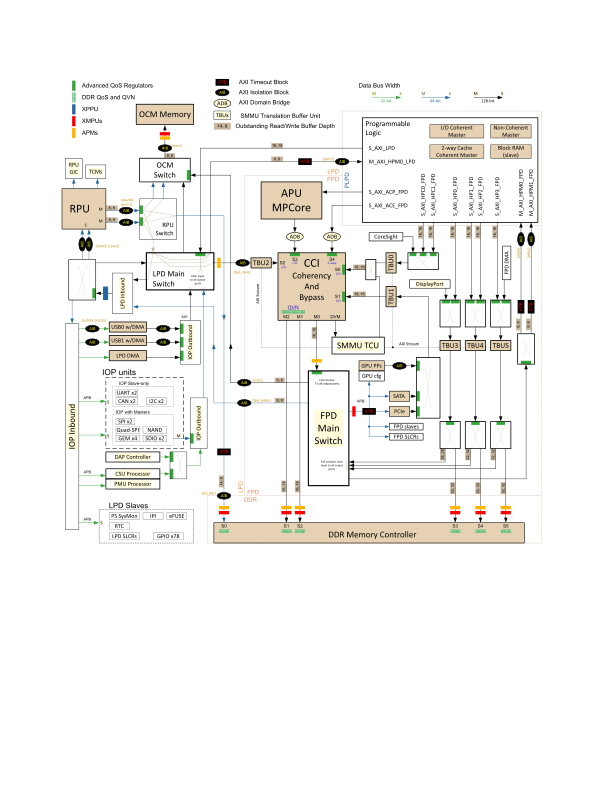
\includegraphics[scale=.9,center,trim={0 75mm 0 0},clip]{img/zynqmp.pdf}
  \caption{The Zynq UltraScale+ system architecture, image from Xilinx \cite{ug1085}.
  The naming nomenclature denotes (in order) the master or slave role, 
  the protocol (AXI), the port name with the modifier ``C'' for ``coherent'' or
  repeating ``M'' for ``master'' then followed by the port number, and finally
  the power domain designation.
  }
  \label{fig:zynqmp-interconnect}
\end{figure}


\subsubsection{High Performance Ports}
\label{sect:implementation}

The UltraScale+ features four \gls{hp} ports that reside in the \glsentrylong{fpd}.
As one can realize from figure \ref{fig:zynqmp-interconnect},
the path from an \gls{hp} port to the memory controller is not identical for all ports.
Indeed, the memory port S3 is shared between the HP0 and the DisplayPort controller
while the S5 is shared between HP3 and the \gls{fpd} DMA.
The interfaces HP1 and HP2 share exclusive access to memory port S4,
a property to be considered if the lowest latency 
or a deterministic performance is desired. Additionally, if the DisplayPort
controller is not used, the HP0 will have full bandwidth access to the S3 memory port.
The HP3 would be the least attractive to use, 
since the memory access pattern of the \gls{fpd}
DMA may not always be known in advance.

\subsubsection{High Performance Coherent Ports}

As the name suggests, the \gls{hpc} ports are cache-coherent versions of \gls{hp}, 
albeit \glslink{IO Coherency}{IO coherent} only, much like the \gls{acp} port. 
However, in contrast to the \gls{acp},
the coherency is not ensured by the \gls{scu} but by the \gls{cci}.

Decoupling the port from the processor has both its benefits and its shortcomings. 
The \gls{hpc} ports have higher latency than \gls{acp} to the memory controller,
even higher than \gls{hp} ports since they have to cross \gls{cci}.
On the other hand, it does not share a path with the processor to the cache,
alleviating the resource competing in a such an important pathway.
Xilinx labels the \gls{acp} as a ``legacy'' port, 
showing its preference in \gls{hpc}.

There are two such ports in UltraScale+. They share access to a single
port of the \gls{cci}, which they can reach after crossing two switches.
From there, they can be routed to the two memory ports that are visible
to the \gls{cci}.

\subsubsection{High Performance Master Ports}

Essentially, the \gls{hpm} ports inherit the role of Zynq-7000's \gls{mgp} ports.
They are masters to the PL, so they are the gateway for any traffic generated with
the initiative of the PS, that being the ARM cores or the PS DMA controllers.

There are three such ports. Two of them are in the \gls{fpd} and one in the \gls{lpd}.
Unlike Zynq-7000, their performance is not inferior to \gls{hp} ports.

\subsubsection{The AXI Slave Port of LPD}

There is a single slave AXI port that connects the PL to the \acrlong{lpd}.
The port is connected to the LPD Main Switch, and from there is routed to the \gls{rpu}
after crossing two further switches. 
Along with the \gls{lpd} \gls{hpm}, 
they are the only means of accessing the PL from
\gls{rpu} side without crossing the \acrlong{fpd}.


\subsubsection{Accelerator Coherency Port}

Retained albeit unfavored from the Zynq-7000 series, the \gls{acp} port
is upgraded to match the performance of the other UltraScale+ ports.
Only one such a port is available.

\subsubsection{AXI Coherency Extensions Port}

The \gls{ace} port is a unique addition to this FPGA-SoC family. 
With the help of \gls{cci} it can offer two-way, full cache coherency.
That is, it can support a cache-enabled peripheral and maintain coherency of both
the processor's and the peripheral's cache.

\section{Exchanging Data with the Programmable Logic}

The diversity of the physical interconnect creates a number of 
possible methods for transferring data between PS and PL.
Each method may benefit a specific transfer pattern or may be more appropriate for an application.
The temporal characteristics of the transfer, the amount of data to be transmitted, 
the requirements for latency or throughput, 
the power consumption and the need of a higher level of determinism,
all of them will derive the optimal solution for each problem.

\subsection{Programmed I/O from a Processor}

The Zynq 7000 features two ARM Cortex-A9 processor cores
that can generate load/store requests. These may target
the DDR memory and the \gls{ocm} directly from the cache ports
and the \gls{scu} respectively, or the PL through the means
of Master Interconnect (see \ref{fig:zynq7000-interconnect}).1

The UltraScale+ is a bit more complicated since it features
two processor clusters that use different pathways.
The high-power A53 cores in \gls{apu} are connected to the \gls{cci}
and from there they may reach either the DDR memory controller,
or be routed from FPD Main Switch either to one of the \acrlong{hpm}s to reach the PL,
or the OCM Switch to reach the \gls{ocm}.
The low-power R5 in \gls{rpu} can only send to the RPU Switch.
From there it can reach three targets: 
The OCM Switch that provides access to the \gls{ocm},
the DDR memory controller directly,
and the \gls{lpd} \gls{hpm} that gives access to the PL.
Additionally, it has a link to the \gls{cci} through the LPD Main Switch
from where it can be routed anywhere in the \acrlong{fpd}, including the \gls{fpd} \glspl{hpm}.

Overall, the main advantage should already be obvious:
The Programmed I/O method can low-latency access to any component of the PS and the PL,
without the need of any PS or PL third-party actor, like a DMA controller. Thus, it saves
resources on both PS and PL.

The second big advantage is simplicity. From software point of view, 
it is sufficient that the program issues the appropriate load / store instructions,
with a possible memory barrier -- no initialization of any component.
As for hardware, an slave peripheral is sufficient to
implement an \gls{axilite} interface, which is low demanding in complexity and resources.

The major drawback derives from the very nature of programmed I/O and is not Zynq specific.
The fact that the traffic is generated by load / store instructions is a twofold problem:
First it keeps the processor busy issuing the instructions preventing it 
to perform any other useful work. The problem aggravates as the number of slaves increases,
as obviously there cannot be more parallel transfers than the number of processors executing I/O.
Secondly, the load / store instructions cannot generate \gls{burst} transfers,
essentially degenerating a full \gls{axi} to \gls{axilite}. 
According to Xilinx (\cite{ug585}, v1.11, pg. 656) one should expect 
transfer rates of around 25MB/s in Zynq-7000.

The most common use case for this method is writing configuration registers,
reading status or other initialization work. 
Such small data exchanges are latency sensitive, not throughput,
making a perfect fit for programmed I/O.

\subsection{Using the ``hard'' DMA controller in the PS}

The Zynq-7000 features an eight-channel DMA controller on the PS side.
Looking back at figure \ref{fig:zynq7000-interconnect} we can see that it is connected
with a single link to the Central Interconnect. 
From there, it may reach the DDR Controller directly, the \gls{ocm} memory through the
OCM Interconnect, and finally, through the Master Interconnect, it may reach the PL by
using one of the \glspl{mgp} (the coarsely dashed line). 

The UltraScale+ has two DMA controllers, one in the \glsentrylong{fpd} and one
in the \glsentrylong{lpd}. 
The \gls{fpd} DMA controller shares a link with the \gls{hp}3. The link
is driven to a second switch that gives access to either the DDR memory controller,
or it is routed to the FPD Main Switch, in turn to the OCM Switch, and finally the \gls{ocm}.
The \gls{lpd} DMA controller is connected to the I/O Peripheral Outbound Switch that is
connected to the LPD Main Switch. From there it can see the OCM Switch and the \gls{ocm} memory,
the DDR memory controller, or it can enter the PL via the LPD \gls{hpm}.

The DMA controllers can be programmed by a PS processor. The programming of a DMA controller
is certainly a more complex matter than just issuing a load / store instruction,
so an increase of software complexity is for granted. 
However, the obvious advantage is that they come ``for free'', that is,
they are already present in the silicon, not consuming any PL resources.
They are multi-channel and they can provide a throughput of at least an order
of magnitude higher than programmed I/O, without keeping busy the processor.

However, as we saw, the flow of data crosses a lot of already busy interconnects.
The sharing of bandwidth reduces all aspects of performance, 
including its predictability and repeatability -- of all users.
We shall not forget also, that even the DMA controllers are actually shared with
other system components, eg the network driver will typically use it to transfer data
to/from the network interface. On top of that, the master ports in both 7000 and UltraScale+
are fewer, and in the former, are also narrower.

Specifically for this work, it should be added that PS DMA is full \gls{axi} compatible
and has no \gls{axistream} -- and neither of the ports of 7000 or UltraScale+ are 
\gls{axistream}-compatible anyway. That means that once the traffic is in the PL,
it must be converted to \gls{axistream}. 
The PL resources needed for this conversion are comparable to implementing a DMA
controller directly to the PL, making this choice appear unattractive.

All in all, the use of the PS DMAs is a viable solution, 
albeit certainly not the best performant. 
To make things worse, it does not map favorably to the goals of this work.
Therefore, this solution was abandoned.

\subsection{Implementing a DMA controller in the PL}

Modern FPGAs are large enough to allow us 
the possibility to implement our own DMA controllers 
at a tolerable cost in PL resources. 

The sacrifice of PL resources is not trivial.
However this drawback could be offset by the number of
advantages that this method gives us:

\begin{itemize}
\item	Both Zynq series feature significantly more 
	slave ports to the PL than master ones.
	Their parallel use would increase aggregate bandwidth.
\item	There is the opportunity to use other interconnect pathways that are not
	being used by the usual client peripherals, alleviating the potential
	issue of an interconnect bottleneck.
\item	Using a path that does not cross the Central Interconnect and the
	Master or Slave Interconnect would have the benefit of 
	reduced and more predictable latency. 
	In the extreme case, one could dedicate a whole pathway 
	for a specific latency critical accelerator.
\item	The PS DMA would be freed for use by other services, 
	especially the network driver.
\item	We gain the flexibility implement the PL DMA
	exactly according to our specific needs.
	It could itself become grounds for research,
	as the capability of the DMA controller
	plays a significant role in overall system performance.
\item	It opens the possibility for the design of more complicated 
	architectures than our case of an isolated accelerator 
	that reads from memory, processes, and writes back.
	For example, output could be re-routed to 
	another accelerator or to an external device
	(ie chip to chip data exchange, data acquisition or data display)
	without the need of going back and forth to the main memory.
\end{itemize}

The choice of slave port however, is a decisive factor 
as it can deny us several of the aforementioned advantages.
Therefore, they should be treated separately.

\subsubsection{The HP ports}

In Zynq-7000 series, the \gls{hp} ports have an 
exclusive access to two memory ports 
through the memory interconnect.
This is an impressive feature, considering that the processor and
the Central Interconnect have only one each.
Furthermore, by having four of them, 
we gain significant flexibility on the AXI interconnect
that it will need to be implemented at the PL side.

Similarly, in UltraScale+, the four \gls{hp} ports have
access to three memory ports, after crossing two rows of switches.

The primary drawback of these ports is that they are not cache-coherent.
In this implementation, the access pattern is a continuous stream of data
that flow through the accelerator. That pattern has zero temporal locality --
caching the data would be useless if not harmful.

Therefore, these ports would be the prime candidates for connecting 
the accelerators.

\subsubsection{The HPC ports (UltraScale+ only)}

The \gls{hpc} ports, in contrast to \gls{hp}, cross the \gls{cci} to reach
the memory controller. This has two side effects: Firstly, they can 
optionally be cache-coherent, and secondly, the crossing of \gls{cci}
will induce a latency penalty.

Eventually, since cache coherency is not important for this implementation,
the \gls{hp} ports would be preferable. However, despite that \gls{hpc} ports
incur a small latency, they offer a path to access two further memory controller
ports, increasing our potential bandwidth by 66\%. 
Therefore, they could be used in addition to the \gls{hp} ports, albeit with
cache coherency disabled.

\subsubsection{The ACP port}

The \gls{acp} port is an interesting addition not only due to its \glslink{IO Coherency}{IO coherent}
nature, but also due to its proximity with the processor. 
The \gls{acp} port would be ideal in an access pattern where the processor and the PL accelerator
work together, exchanging small pieces of data or cooperatively working in the same dataset.
Essentially, the ``accelerator'' would be more of a ``co-processor''.
In this access pattern, the data generated from the processor would stay in cache, from where
the \gls{acp}-connected accelerator will retrieve it, without accessing the DDR memory at all.
This would have a huge benefit to memory throughput and
would alleviate the traffic of the memory controller. Additionally, since retrieving data
from cache is an order of magnitude cheaper in energy than retrieving from memory,
the power efficiency of the system would dramatically improve.

Nonetheless, this is not our case. Our streaming data pattern would 
cause continuous cache misses and cache thrashing,
increasing the latency and depriving the processor any cached memory.
Furthermore, the \gls{acp} and the processor core share the connectivity
of the \gls{scu} to the L2 cache, competing for access.
Performance-wise it would be a disaster and therefore it will not be attempted.

\subsubsection{The ACE port}

The ACE protocol differs from both \gls{hpc} and \gls{acp} 
in that it offers full, two-way coherency. This permits
maintaining cache coherency between the processor with caches and a
full \gls{axi} peripheral with cache in the form of \gls{bram}.

In comparison to \gls{acp}, the \gls{ace} (and also the \gls{hpc}) do not compete
with the processor for cache access. 
Yet, the \gls{ace} adds significant complexity to the slave and the interconnect.
Its access to the memory controller is through the \gls{cci}, an access already
gained through \glspl{hpc}, leaving us little incentive to use this port.

\subsubsection{The S\_GP in 7000 and the LPD Slave AXI in UltraScale+}

In section \ref{sect:sgp} it was described how \gls{sgp} can reach the memory controller.
It is a complex path that comprises crossing both the Slave Interconnect and the Central
Interconnect. That cancels out a couple of our initial arguments for the use of the slave ports.
Further discouraging is the fact that we will compete 
with the \gls{devc} which controls the single \gls{pcap}
port used to reconfigure the FPGA.

Still, the \gls{sgp} will open us access to one more port to the DDR controller.
For this very reason, it is worth to experiment using it.

The LPD Slave AXI port of the UltraScale+ shares some characteristics with \gls{sgp}.
However, studying the figure \ref{fig:zynqmp-interconnect} we will see that the port
can reach the memory controller through the LPD Main Switch and the \gls{cci},
not the RPU Switch, whose only master is the \gls{rpu} itself.
This actually the case even for the LPD DMA.

This was an intended design decision. The \gls{rpu} needs exclusive access to the
memory controller in order to offer predictable and repeatable access latency,
a key characteristic of its real-time nature.

Therefore, there is not much incentive to use it, since we already access the
memory ports of the \gls{cci} via the \glspl{hpc}.

\section{Design Components}

\subsection{The DMA controller}
\label{sec:axidma}

By initial problem statement it was decided that the system will feature
streaming accelerators. This narrows down the DMA controller selection
to AXI DMA and AXI VDMA. The latter is video oriented, offering additional
functionality that is desirable in video applications -- and even required
by some controller cores of imaging peripherals. Our test application
is indeed imaging oriented and would be benefited by AXI VDMA in a few ways.
Firstly, it would enable the possibility of using the Xilinx OpenCV-compatible
HLS video libraries. Secondly, the out-of-band synchronization that is possible
with the VDMA would enable the accelerator to detect when the image line changes
and when the frame ends. Lastly, as VDMA was made for embedded use, it would be
beneficial in case it was decided to bring this system in an embedded setting.

However, the test application is just for testing and not the only intended use.
The loss of generality, or even the increased complexity due to specialization,
was undesired. That leaves us with only the AXI DMA.

The AXI DMA IP core has a few operating modes that are worthy of mentioning.

\begin{itemize}
\item	\textbf{Direct Register}: 
	This is the simplest operating mode. A DMA operation is initiated 
	by writing the control, source and destination registers.
	The processor can query the status register for completion, 
	either by polling or by interrupt notification.
	Operation queuing is not supported, therefore there will be a time gap 
	between completion and re-programming with next operation.
	This operation trades performance for resource utilization.
\item	\textbf{Scatter-Gather}:
	In this mode, the AXI DMA creates an auxiliary \gls{axi} port
	to a memory resource that contains a list of transfer descriptors.
	The AXI DMA will execute sequentially all the descriptors without
	any intermediate pause. Upon completion, it may pause or restart
	executing the same list. This mode offers higher performance 
	as the DMA controller never stalls.
\item	\textbf{Multichannel}: 
	An option to the Scatter-Gather mode,
	that allows multiple virtual channels on the streaming side.
	The AXI DMA will still have only two interfaces and the channels
	will be differentiated by the sideband information that is carried
	over a standard \gls{axistream} channel. This option is interesting
	in that it permits a single DMA controller to handle multiple accelerators.
\end{itemize}

The more complex operating modes show a lot of promise for our intended system.
However, the Direct Register mode was chosen, on the grounds of simplicity
and as a ``starting point''. The potential of the other modes will be
discussed at the ``Future Work'' section.

In table \ref{tab:dma-modes} the resource cost of each operating mode is displayed.

\begin{figure}[ht!]
\centering
\begin{tabular}{ccl c rrrrr}
%\cmidrule[\heavyrulewidth](l{-0.75em}r{-0.75em}){1-8}
\toprule
&	&	&~& LUT& FF	& BRAM	& Nets	\\
\cmidrule(l{.3em}r{.3em}){1-8}
\multirow{10}{*}{\rotatebox{90}{Zynq 7000}}
&\multirow{5}{*}{\rotatebox{90}{32 bit data}}
	& DR	&& 1571	& 1996	& 2/0	& 404	\\
&	& SG	&& 2076	& 3235	& 2/0	& 593	\\
&	& MC 1ch&& 2696	& 3807	& 2/0	& 637	\\
&	& MC 8ch&& 3245	& 4188	& 2/0	& 637	\\
&	& MC 16ch&&3877	& 4626	& 2/0	& 637	\\
\cmidrule(l{.3em}r{.3em}){2-8}
&\multirow{5}{*}{\rotatebox{90}{64 bit data}}
	& DR	&& 1811	& 2394	& 2/2	& 544	\\
&	& SG	&& 2362	& 3636	& 2/2	& 733	\\
&	& MC 1ch&& 2978	& 4208	& 2/2	& 777	\\
&	& MC 8ch&& 3527	& 4589	& 2/2	& 777	\\
&	& MC 16ch&& 4159& 5027	& 2/2	& 777	\\
\midrule
\multirow{10}{*}{\rotatebox{90}{Zynq UltraScale+}}
&\multirow{5}{*}{\rotatebox{90}{32 bit data}}
	& DR	&& 1544	& 2002	& 2/0	& 404	\\
&	& SG	&& 2101	& 3244	& 2/0	& 593	\\
&	& MC 1ch&& 2722	& 3816	& 2/0	& 637	\\
&	& MC 8ch&& 3271	& 4197	& 2/0	& 637	\\
&	& MC 16ch&&3905	& 4636	& 2/0	& 637	\\
\cmidrule(l{.3em}r{.3em}){2-8}
&\multirow{5}{*}{\rotatebox{90}{64 bit data}}
	& DR	&& 1830	& 2403	& 2/2	& 544	\\
&	& SG	&& 2380	& 3645	& 2/2	& 733	\\
&	& MC 1ch&& 3001	& 4217	& 2/2	& 777	\\
&	& MC 8ch&& 3550	& 4598	& 2/2	& 777	\\
&	& MC 16ch&&4184	& 5037	& 2/2	& 777	\\
\bottomrule
%\cmidrule[\heavyrulewidth](l{-0.75em}r{-0.75em}){1-8}
\end{tabular}
\caption{Resource utilization of the AXI DMA core. Configuration: Burst size 16, address width 32b.\\
	LUT: Look-up tables, FF: Flip-flops, BRAM: Block RAM (36kb/18kb), Nets: Boundary crossing nets.\\
	DR: Direct Register, SG: Scatter-Gather, MC: Multi-channel, $n$-ch: number of channels}
\label{tab:dma-modes}
\end{figure}

As a final note, it should be mentioned that each AXI DMA core outputs two reset signals,
one for the MM2S and one for the S2MM channel, that are asserted when the corresponding channel is also rest.
It also outputs two interrupt signals, again, one for each channel. 
The Zynq-7 has an interrupt input of 16 bits and Zynq UltraScale+ has two 8-bit inputs.
The maximum number of AXI DMA that could be directly connected would be 8, which is very restrictive.

For the Zynq-7, a workaround approach was employed. We only use the S2MM interrupt output,
and we ``lie'' at the operating system about MM2S. This is mandatory, as the Xilinx DMA driver requires
both interrupts to be defined. In our kernel driver however, the DMA client to the Linux API takes
care \emph{not} to query or place any callback function on MM2S interrupt, and considers the transfer done
when the S2MM interrupt is asserted. With this workaround, we raise the maximum number of AXI DMA instances
to 16, which were sufficient given the Zedboard's FPGA size.

For the Zynq UltraScale+, this does not suffice, as its size enables the instantiation of much more than 16
AXI DMAs. Therefore, in our port, we made use of the AXI Interrupt Controller IP Core, which supports up
to 32 interrupts per instance. The Zynq-7 workaround was still used, in order to reduce the interrupt
controller instance count and to avoid instantiating unnecessary wires.

\subsection{The Interconnect}

The choice of PL interconnect is a trade-off between several important metrics.
The interconnect must match the required clock. 
Using register slices to pipeline the \gls{axi} channels is useful, 
but may not suffice if the critical path is within the switching logic.

A large and complex interconnect, one that connects many slaves to many masters
may achieve maximum flexibility but will likely become the clock bottleneck,
drastically reduce design routability and consume significant FPGA resources.

As an attempt to break down complex interconnects, both Zynq families
offer multiple ports for pathways that will most 
probably host a large number of peripherals.
The ports have either a silicon implemented switch that,
from FPGA designer's perspective, comes ``for free'' or they are routed to
another memory port. 

In order to explore the potential solutions, a test design was created for UltraScale+. 
It features eight accelerators that transfer data with 16 unidirectional links. 
We will then experiment on which interconnect will best match our needs.

Note that Xilinx does offer very detailed mathematical formulas 
for estimating resource utilization of each component of AXI Interconnect 
in 7-series FPGAs (see \cite{pg059}, pp 35-52).

\subsubsection{A Naive Solution and Basic Configuration}

Let us begin with using a single AXI Interconnect v2.1
with 16 slave interfaces (SI) and 1 master interface (MI), 
connected to a single \gls{hp} port. The initial configuration
will be a 32b data width crossbar, outer register slices in all interfaces,
as well as a 32 byte FIFO.

The first thing to notice in this basic design,
it that with the default memory map, the PL has access not only to the DDR,
but also to PCIe, QSPI and OCM address spaces. 
This is made possible by appending an AXI MMU core on each slave interface.
As it can be seen on table \ref{tab:int-mmu}, eliminating this unused flexibility
reduces lightly the resource usage. Other tweaks, like the map base or range
have negligible effect.

Note that the ``Nets'' column refers to the core's boundary crossing nets,
and is a metric that predicts routability.

\begin{figure}[ht!]
\centering
\begin{tabular}{lrrr}
\toprule
			& LUT	& FF	& Nets \\
\cmidrule(l{.3em}r{.3em}){1-4}
DDR, PCIe, QSPI, OCM	& 3002	& 5466	& 1792\\
DDR only		& 2883	& 5430	& 1792\\
\bottomrule
\end{tabular}
\caption{The effect on memory map on resource utilization and routability.\\
	Configuration: AXI Interconnect v2.1, 16 SI / 1 MI, 32 bit crossbar, 
	outer register and 32 byte FIFO per port.}
\label{tab:int-mmu}
\end{figure}

The next challenge would be other two coupler components, the register slices
and the FIFO buffer. The register slices are applied to all five channels of the full \gls{axi},
albeit using different structures (for details, see \cite{pg059} pg 93).
The optional FIFO buffer may be implemented in \gls{lutram} as 32-deep or in \gls{bram} 
as 512-deep. The latter option will also add 32-deep FIFOs to address channels.
Table \ref{tab:int-reg} shows the effect of these options.

\begin{figure}[ht!]
\centering
\begin{tabular}{lrrr}
\toprule
	& LUT	& FF	& Nets \\
\cmidrule(l{.3em}r{.3em}){1-4}
No register slices, no FIFO		& 1337 & 526 & 1792 \\
No register slices, 32-deep FIFO	& 2362 & 2800 & 1792 \\
No register slices, 512-deep FIFO	& 4459 & 7967 & 1792 \\
Outer register slices, no FIFO		& 1858 & 3156 & 1792 \\
Outer register slices, 32-deep FIFO	& 2883 & 5430 & 1792 \\
\bottomrule
\end{tabular}
\caption{The effect of register slices and FIFOs on AXI Interconnect implementation size.\\
	Configuration: AXI Interconnect v2.1, 16 SI / 1 MI, 32 bit crossbar}
\label{tab:int-reg}
\end{figure}

Apparently, these couplers take up the lion's share of the total interconnect resources.
Their importance however, differs greatly. 
The register slices, despite the fact they cause a rise of about 40\% in LUT usage,
during the development of the high core count design,
they were found to permit a 10 to 20\% higher clock in a congested circuit. 
\emph{TODO: μπορώ να το πω αυτό;}
Their cost was therefore justified. 
The FIFO however is mostly useful when data or clock conversion occurs in the
interconnect. Therefore, the 32-deep version might be used if the overall design
has sufficient free LUTs. The 512-deep version however,
not only dramatically increases resource usage, but also places area constraints on
the design since \glspl{bram} are found in specific areas, that at least in Zynq-7000
are scarce, since \gls{bram} is also required by both the AXI DMA and our reconfigurable
partitions in order to implement the convolution line buffer.
\\

Presumably, the most important parameter of an interconnect would be its data channel's width. 
The width should match both that of the peripheral's and of the Zynq's connecting port.
Table \ref{tab:int-width} demonstrate its effect on implementation size.

\begin{figure}[ht!]
\centering
\begin{tabular}{lrrr}
\toprule
	& LUT	& FF	& Nets \\
\cmidrule(l{.3em}r{.3em}){1-4}
32 bit	& 2883	& 5430	& 1792 \\
64 bit	& 3777	& 7942	& 2404 \\
128 bit	& 5605	& 12966	& 3628 \\
\bottomrule
\end{tabular}
\caption{The effect of the AXI Crossbar width on AXI Interconnect implementation size.\\
	Configuration: AXI Interconnect v2.1, 16 SI / 1 MI, outer reg slices and 32-deep FIFO}
\label{tab:int-width}
\end{figure}

Therefore, the resource utilization does increase, but there is little we can do.
It is a parameter normally decided by the data width of the accelerator.
If we manually override the crossbar width, the AXI Interconnect will place
data width converters in all interfaces where the remote endpoint of the channel disagrees.

Here comes a significant pitfall in the Vivado tool. The crossbar width is inherited
from the endpoint that connects to the Master Interface. In our case, the UltraScale+'s \gls{hp} port.
By default, these ports will be defined with the maximum possible value, i.e. 128 bits.
The Slave Interfaces of AXI Interconnect are driven by the AXI DMA controllers,
whose memory mapped channel's data width are inherited by the data width of the AXI stream,
which is decided by the accelerator. Note that AXI DMA will not allow a data width of less
than 32 bits despite that it allows a stream data width down to 8 bits.

It is unlikely these values would match; data width converters would be instantiated by
the AXI Interconnect, leading to severe increase in resource utilization.
To illustrate this, the table \ref{tab:int-dw} shows the effect of using the default
settings when connecting a 32-bit accelerator to a 64-bit port (Zynq-7000 default)
or 128-bit port (UltraScale+ default).

A special case that arose during the development of the UltraScale+ port,
is the \gls{axilite} peripheral control interconnect. 
If the IP core is automatically placed by Vivado Block Automation,
it is instantiated with a data width converter on its single slave interface
and the crossbar hierarchy is implemented in 32 bits.
However, if it is manually placed, the data width converter will be placed
at the slave interfaces of all tier-2 crossbars, while the tier-1 crossbar will be
at the port width, i.e. 128 bits. 
This effect, in our case, lead to a comparative 2.5x increase in LUT and 2x increase in FF utilization.


\begin{figure}[ht!]
\centering
\begin{tabular}{lrrr}
\toprule
			& LUT	& FF	& Nets \\
\cmidrule(l{.3em}r{.3em}){1-4}
32 bit SI, 32 bit MI	& 2883 & 5430 & 1792 \\
32 bit SI, 64 bit MI	& 5421	&5286	&1826	\\
32 bit SI, 128 bit MI	& 8053	&8214	&1962	\\
\bottomrule
% for 128 bits smartconnect &4231   &8389   &2368 pg
\end{tabular}
\caption{The effect of master-slave data width mismatch on AXI Interconnect implementation size.\\
	Configuration: AXI Interconnect v2.1, 16 SI / 1 MI, outer reg slices and 32-deep FIFO}
\label{tab:int-dw}
\end{figure}

Unless this is desirable (e.g. to increase the maximum port throughput),
it is advisable to configure the Zynq port at identical data width with the
full \gls{axi} ports of AXI DMA.

\subsubsection{Attempting Parallel Access to Memory}

Since both Zynq families offer multiple PS-PL ports that lead to 
multiple memory ports of the memory controller,
it is an opportunity for access parallelization.

However, in section \ref{sect:zynq7000-hp} 
\emph{[TODO να βρω την ταχυτητα της θυρας DDR του US+]} 
we saw that, regarding Zynq-7000,
the aggregate throughput of just two \gls{hp} ports
is sufficient to saturate the memory controller, 
even if we do not take into account its other potential users, 
e.g. the processor or the I/O peripherals.
Given the comparatively low throughput of the Zynq-7000 memory subsystem,
one may wonder if there is sufficient motivation for even attempting parallelization.
There are two arguments in favor of doing it -- and virtually none against.

Firstly, the maximum theoretical throughput of 2400MB/s that Xilinx asserts (\cite{ug585}, pg 652)
was calculated assuming maximum port frequency, maximum port width, and continuous bidirectional
traffic. The latter is unlikely, but there is little we can do. As for the other two,
they are subject to design trade-offs between per-accelerator performance vs. accelerator count
and lower values might be chosen, effectively operating the port at a fraction of its
maximum rate. At the PS side however, the memory interconnect and the memory controller
operate in separate clock domains and with fixed width ports,
so their maximum throughput is undifferentiated by the PL design.

Secondly, the complexity of the interconnect might limit the maximum attainable clock.
Breaking down a single big interconnect to several smaller will allow a far better
	\footnote{
		According to \cite{pg059} pg 23, for Artix-7 class FPGAs, 
		like the smaller members of Zynq-7000 family, the maximum attainable
		clock for speed grade 2 devices is 130MHz for a 64b interconnect of
		16 slave / 1 master interfaces, and 205MHz for a 4 slave / 1 master.
	}
maximum clock.

Therefore, the parallelization is worth of exploring, the only question is
which is the best architecture for our purpose.

Intuition would command us to increase the number of AXI Interconnect
Master Interfaces. Granted, it violates our second argument, but since
it is the simplest architecture and actually the first that was attempted
in this work, it is worth of assessing it.

This configuration will complicate the processor memory map
since a peripheral must be able to reach a processor address using
exactly one possible route. 
This could be solved by segmenting the processor memory
and offsetting the burden of access parallelization to the software,
in the sense that if software chooses the memory buffers properly
it can balance the \gls{transaction} rates between all ports.

What cannot be solved however, is the hardware cost that arises of the increased
complexity, as it is shown in table \ref{tab:int-mmi}.

\begin{figure}[ht!]
\centering
\begin{tabular}{lrrr}
\toprule
	& LUT	& FF	& Nets \\
\cmidrule(l{.3em}r{.3em}){1-4}
1 MI	& 2883	& 5430	& 1792	\\
2 MI	& 3590	& 6195	& 2046	\\
3 MI	& 4044	& 6912	& 2300	\\
4 MI	& 4849	& 7641	& 2554	\\
\bottomrule
\end{tabular}
\caption{The effect on master interface count on AXI Interconnect resource utilization and routability.\\
	Configuration: AXI Interconnect v2.1, 16 SI / 1 MI, 32 bit crossbar, 
	outer register and 32 byte FIFO per port.}
\label{tab:int-mmi}
\end{figure}

The resource increase is significant but not prohibitive. 
However one could see a source of redundancy: Even if the problem
of accessing a memory address by multiple routes can be solved by segmentation,
it would be better if the redundant paths were not available at all.
This would not only simplify software, but most importantly we would expect
a simplification of the interconnect.

The solution is to break up the interconnect to several smaller. 
A 16 SI / 4 MI interconnect could be
broken to four 4 SI / 1 MI interconnects. 
This would yield several advantages:
\begin{itemize}
\item	Avoidance of segmentation would lead to software simplification.
\item	The removal of redundant paths is expected to reduce interconnect resource utilization.
\item	An interconnect with fewer SI or MI interfaces can work in higher clock speeds.
\item	It opens the way of asymmetric access to memory, including exclusive memory access
	for reconfigurable partitions hosting time-critical accelerators.
\end{itemize}
 
A secondary question would be how to split the interconnect. 
For example, if we decide to split the interconnect by two, 
would we split it by assigning half of the DMA controllers to the first
part of the interconnect and half to the second, or it might be a better idea to split by
channel type, given that read and write channels are significantly different? 
In order to answer this, a design with two 8 SI / 1 MI interconnects was created.
At first the AXI DMA were split equally and later split by interface type.
The results are in table \ref{tab:int-mixed}.

\begin{figure}[ht!]
\centering
\begin{tabular}{lrrr}
\toprule
			& LUT	& FF	& Nets \\
\cmidrule(l{.3em}r{.3em}){1-4}
Split equally 		& 3060	&6290	&2044 	\\
Split by interface type	& 2787	&6006	& 2044	\\
\bottomrule
\end{tabular}
\caption{The effect of SI type homogeneity on AXI Interconnect resource utilization and routability.\\
	Configuration: AXI Interconnect v2.1, 2x 8 SI / 1 MI, 32 bit crossbar, 
	outer register and 32 byte FIFO per port.}
\label{tab:int-mixed}
\end{figure}

Now, we can proceed to explore three interconnect architectures.
The table \ref{tab:int-msi} reveals the resource utilization for each one.

\begin{figure}[ht!]
\centering
\begin{tabular}{cl rrr}
\toprule
&		&Logic LUT & FF	& Nets \\
\cmidrule(l{.3em}r{.3em}){1-5}
\multirow{3}{*}{\rotatebox{90}{32 bit}}			
&1 I/C of 16 SI	& 2883	& 5430	& 1792 	\\
&2 I/C of 8 SI	& 2787	& 6006	& 2044	\\
&4 I/C of 4 SI	& 3282	& 7420	& 2544	\\
\cmidrule(l{.3em}r{.3em}){1-5}
\multirow{3}{*}{\rotatebox{90}{64 bit}}
&1 I/C of 16 SI	& 3777	& 7942 	& 2404	\\
&2 I/C of 8 SI	& 3759	& 8790	& 2724	\\
&4 I/C of 4 SI	& 4400	&10812	& 3360	\\
\cmidrule(l{.3em}r{.3em}){1-5}
\multirow{3}{*}{\rotatebox{90}{128 bit}}
&1 I/C of 16 SI	& 5605	& 12966	& 3628	\\
&2 I/C of 8 SI	& 5656	& 14359	& 4084	\\
&4 I/C of 4 SI	& 6874	& 17604	& 4992	\\
\bottomrule
\end{tabular}
\caption{Effect of interconnect architecture on resource utilization and routability.\\
	AXI Interconnect: Outer register and 32-byte FIFO for each port.}
\label{tab:int-msi}
\end{figure}

Apparently, splitting up the interconnect proved to only marginally increase
resource utilization, essentially giving us all the aforementioned advantages at almost no cost.


\subsubsection{Comparing AXI Interconnect and SmartConnect}

In 2016, Xilinx released a new IP core that implements 
the functionality of a Full \gls{axi} interconnect,
claiming remarkably higher maximum clock at UltraScale+ devices.

During the hardware design development, the new IP core was put to test.
The maximum clock frequency was sought in a moderately congested design,
using a static workflow but with all partial reconfiguration related 
\gls{pblock} placement constraints enabled. The end result was that
using SmartConnect a clock of 143MHz was achieved, whereas with
AXI Interconnect only 125MHz could be attained.

Unfortunately, this achievement came at the expense of resource utilization.
As the increase was significant, it was deemed necessary to quantify the overhead.
The table \ref{tab:smartconnect} summarizes the results of implementing 
a test-case of a single 16 SI / 1 MI interconnect implemented with both the 
AXI Interconnect and the SmartConnect, in both Zynq-7000 and UltraScale+ devices.

\begin{figure}[ht!]
\centering
\resizebox{\textwidth}{!}{%
\begin{tabular}{ccl rrr c rrr}
\toprule
&&				& \multicolumn{3}{c}{Zynq 7000} & ~ & \multicolumn{3}{c}{Zynq UltraScale+}\\
&&				& LUT	& FF	& Nets 	&& LUT 	& FF 	& Nets	\\
\cmidrule(l{.3em}r{.3em}){1-10}
\multirow{4}{*}{\rotatebox{90}{Single 16-MI }}
&\multirow{2}{*}{\rotatebox{90}{32 bit}}
&AXI Interconnect v2.1		&3305 & 5877 & 1756	&&2883 	&5430	&1792	\\
&&SmartConnect v1.0		&12910	&9381	&1777	&&14151	&10835	&1817	 \\
\cmidrule(l{.3em}r{.3em}){2-10}
&\multirow{2}{*}{\rotatebox{90}{64 bit}}
&AXI Interconnect v2.1		&4231	&8389	&2368	&& 3777	&7942	&2404	\\
&&SmartConnect v1.0		&15605	&12351	&2429	&&15605	&12351	&2429	 \\
\cmidrule(l{.3em}r{.3em}){1-10}
\multirow{4}{*}{\rotatebox[origin=r]{90}{ Quad 4-MI}}
&\multirow{2}{*}{\rotatebox{90}{32 bit}}
&AXI Interconnect v2.1		&4914	&9150	&2392	&& 3282	&7420	&2544	\\
&&SmartConnect v1.0		&13748	&10470	&1972	&& 12998&9920	&2052 \\
\cmidrule(l{.3em}r{.3em}){2-10}
&\multirow{2}{*}{\rotatebox{90}{64 bit}}
&AXI Interconnect v2.1		&6082   &12542  & 3208	&& 4400	& 10812	& 3360	\\
&&SmartConnect v1.0		& 15046	& 12154	&2652	&& 14404& 11608 & 2732\\
\bottomrule
\end{tabular}
}
\caption{Comparison of AXI Interconnect and AXI SmartConnect, on 7000 and UltraScale+.\\
	AXI Interconnect v2.1 vs AXI SmartConnect v1.0, 4 instances of 4 SI / 1 MI, 32 bit crossbar.\\ 
	Configuration: Outer register and 32 byte FIFO per port.}
\label{tab:smartconnect}
\end{figure}

Apparently, the 15\% gain in clock speed was accompanied by a threefold increase in LUT utilization. 
Therefore, its use may not be recommended in the following cases:

\begin{itemize}
\item	If area is at a premium and functional completeness cannot be achieved with SmartConnect.
\item	If the critical path resides inside the accelerator core.
\item	For the \gls{axilite} peripheral control interconnect. Either way, \gls{axilite} peripherals
	cannot be clocked as high as full \gls{axi} or \gls{axistream} ones.
	\footnote{For the AXI DMA case, the figure is actually around 25\% 
	lower (see \cite{pg021}, pg 8).} Given that configuration
	ports, the typical users of \gls{axilite}, are not performance critical, it would be
	better that the \gls{axilite} paths reside in a separate (lower) clock domain.
\end{itemize}

\section{The Implemented Designs}

Taking into account all these observations, an architecture had to be designed.
Firstly, the design objectives must be stated:

\begin{itemize}
\item	\textbf{Correctness}:
	The design will be the means to prove that the proposed system does work.
	It shall function properly for any user input data within its specifications
	and process it in a timely manner.
\item	\textbf{Flexibility}: 
	The software (i.e. the kernel driver) shall support,
	without recompilation or additional user intervention,
	any possible interconnect architecture and memory topology
	as long as it is properly described in the \gls{dt}.
	An accelerator may have a restricted view of the addressable memory space
	or might be given exclusive access to a certain region.
	The memory space itself might be a collection of different memory resources
	with unequal proximity to the programmable logic. 
	The designer must be able to explicitly express a relative preference 
	to one resource against another.
\item	\textbf{Performance}:
	The design will implement an efficient interconnect that enables 
	parallel memory access for the accelerators. 
	Its architecture must permit sufficiently high clock speeds.
	Finally the final system will show the performance of partial reconfiguration
	as well as the flexibility of the accelerator scheduler.
	However, we will not explore the optimal architecture for solving any specific problem.
\item	\textbf{Portability}:
	A constant effort throughout both hardware and software design was that they should be
	as decoupled as possible. The software shall use standardized operating system
	interfaces to ensure that porting the system to a different would be done with
	least effort possible.
\end{itemize}

In order to pursue these objectives, three designs were developed.

\subsection{An Accelerator Performance Oriented Approach}

The first design is geared to accelerator performance, featuring
accelerators with wider interconnect that allow
greater data processing parallelization.
It has homogeneous reconfigurable partitions with
full memory view of uniform access on the accelerator side, 
allowing total freedom of accelerator placement that
maximizes the scheduler's decision options.

\begin{figure}[ht!]
\centering
\hspace{-15mm}
\begin{tikzpicture}

	% Border
	\draw[dotted] (-40mm,0) -- node[above left = 0mm and 50mm]{PL} node[below left = 0mm and 50mm]{PS} (80mm,0);
	
	% The PS-PL ports
	\node[port] (hp0) at (-16mm,0) {\ttfamily HP0};
	\node[port] (hp3) at ($(hp0) + (32mm,0mm)$) {\ttfamily HP3};
	\node[port] (hp1) at ($(hp0)!0.333!(hp3)$) {\ttfamily HP1};
	\node[port] (hp2) at ($(hp0)!0.667!(hp3)$) {\ttfamily HP2};

	\node[port] (plint) at ($(hp3) + (16mm,0mm)$) {\ttfamily INT};

	\node[port] (mgp0) at ($(plint) + (20mm,0mm)$) {\ttfamily M\_GP0};
	\node[port] (mgp1) at ($(mgp0) + (12mm,0mm)$) {\ttfamily M\_GP1};
	
	% The Memory Interconnect
	\node[block, minimum width = 50mm] (mem-interconnect) 
		at ($(hp0)!0.5!(hp3) - (0,20mm)$) {Memory\\Interconnect};
	\draw[axi64] ($(mem-interconnect.south west)!0.1!(mem-interconnect.south east)$) 
		|- node[below left=0mm and -3mm]{\ttfamily\scriptsize OCM Switch} +(-8mm, -4mm);


	% HP to Memory Interconnect
	\draw[axi64, name path=hp0p] (hp0) -- (hp0 |- mem-interconnect.north);
	\draw[axi64, name path=hp1p] (hp1) -- (hp1 |- mem-interconnect.north);
	\draw[axi64, name path=hp2p] (hp2) -- (hp2 |- mem-interconnect.north);
	\draw[axi64, name path=hp3p] (hp3) -- (hp3 |- mem-interconnect.north);

	% Lines internal to Memory Interconnect
	\draw[gray, from end of path=hp0p, name path=mem0p] 
		-- ($(mem-interconnect.south west)!0.28!(mem-interconnect.south east)$);
	\draw[gray, from end of path=hp1p] 
		-- ($(mem-interconnect.south west)!0.28!(mem-interconnect.south east)$);
	\draw[gray, from end of path=hp2p, name path=mem1p] 
		-- ($(mem-interconnect.south west)!0.73!(mem-interconnect.south east)$);
	\draw[gray, from end of path=hp3p] 
		-- ($(mem-interconnect.south west)!0.73!(mem-interconnect.south east)$);

	% Memory controller and DDR box
	\node[block, minimum width=50mm,minimum height=12mm,align=left,text width=29mm, below=12mm of mem-interconnect] 
		(mem-controller) {Memory\\Controller};
	\node[block, minimum width=8mm, minimum height=7mm,right=-15mm of mem-controller] (ps-ddr) {DDR3};

	% From Memory Interconnect to Memory Controller (uses constants!)
	\draw[axi64, from end of path=mem0p] -- +(0,-12mm);
	\draw[axi64, from end of path=mem1p] -- +(0,-12mm);

	% PL Interconnect
	\node[interconnect] (int0) at ($(hp0) + (0, 20mm)$) {};
	\node[interconnect] (int1) at ($(hp1) + (0, 20mm)$) {};
	\node[interconnect] (int2) at ($(hp2) + (0, 20mm)$) {};
	\node[interconnect] (int3) at ($(hp3) + (0, 20mm)$) {};
	\draw[axi64] (int0) -- (int0 |- hp0.north);
	\draw[axi64] (int1) -- (int1 |- hp1.north);
	\draw[axi64] (int2) -- (int2 |- hp2.north);
	\draw[axi64] (int3) -- (int3 |- hp3.north);
	\node[emptyblock, gray, very densely dashed, anchor=north west, minimum width=50mm, minimum height=28mm]
		(axi-int) at ($(int0.north west) + (-5mm, 13mm)$) {};
	\node[textonly, left of=axi-int, xshift=-18mm, rotate=90]{\footnotesize 64b Full AXI Interconnects};

	% The AXI DMA multi-block
	\node[mblock, minimum width = 50mm, minimum height = 16mm] (axidma) 
		at ($(int0)!0.5!(int3) + (0, 40mm)$) {64 bit AXI DMA};
	\node at ($(axidma.north east) + (2mm,2mm)$) {\ttfamily x6};
	
	% Connection of AXI DMA to AXI Interconnect blocks
	\draw[maxi64] (int0 |- axidma.south) 
		node[above]{\texttt{MM2S}}
		node[above left,rotate=90]{\texttt{\small 0..5}} 
		-- 
		node[below left,rotate=90]{\texttt{\small 0..2}} (int0);
	\draw[maxi64] (int0 |- axidma.south) 
		-- +(0,-6mm) -| 
		node[above left]{\texttt{\small 3..5}}
		(int2);
	\draw[maxi64] (int3 |- axidma.south)
		node[above]{\texttt{S2MM}}
		node[above left,rotate=90]{\texttt{\small 0..5}}
		-- node[below left,rotate=90]{\texttt{\small 0..2}} (int3);
	\draw[maxi64] (int3 |- axidma.south) -- +(0,-12mm) -|
		node[above right]{\texttt{\small 3..5}} (int1);

	% The Accelerators
	\node[mblock, minimum width = 50mm, minimum height = 16mm, above=16mm of axidma] (acc) {64 bit Accelerator};
	\node at ($(acc.north east) + (2mm,2mm)$) {\ttfamily x6};

	\draw[raxis64] ($(acc.south west)!0.25!(acc.south east)$) 
		node[above]{\texttt{IN}}
		--($(axidma.north west)!0.25!(axidma.north east)$);
	\draw[axis64] ($(acc.south west)!0.75!(acc.south east)$)
		node[above]{\texttt{OUT}}
		--($(axidma.north west)!0.75!(axidma.north east)$);


	% The Master Interconect
	\node[block, minimum width = 50mm] (master-interconnect) at ($(mgp0)!0.5!(mgp1) - (0,20mm)$) 
		{Master Interconnect\\for Slave Peripherals};

	% M_GP to Master Interconnect
	\draw[raxi64] (mgp0) -- (mgp0 |- master-interconnect.north);
	\draw[raxi64] (mgp1) -- (mgp1 |- master-interconnect.north);

	% APU
	\node[block, minimum width = 50mm, minimum height = 12mm, anchor = north west] (apu)
		at ($(master-interconnect.south west) - (0,12mm)$) {APU};
	\draw[axi64] (apu) -- (apu |- master-interconnect.south);
	\draw[axi64] (apu) -- (mem-controller);

	% The Interrupt
	\draw[-,postaction={decorate}] ([yshift=2mm]axidma.south east) 
		node[below right] {\ttfamily\scriptsize 6}
		node[above right]{\ttfamily\scriptsize S2MM Interrupt}
		-| ([xshift=2mm]plint.north west);
	\draw[-] ([xshift=2mm]plint.south west)
		|- ([yshift=-2mm]apu.north west);

	% Peripheral Interconnect
	\node[interconnect] (per-int0) at ($(mgp0) + (0, 20mm)$) {};
	\node[interconnect] (per-int1) at ($(mgp1) + (0, 20mm)$) {};
	\draw[raxi32] (per-int0) -- (per-int0 |- mgp0.north);
	\draw[raxi32] (per-int1) -- (per-int1 |- mgp1.north);
	\draw[maxil] (per-int0) 
		node[above right, rotate=90]{\ttfamily \textcolor{black}{~~0..5}}
		|- node[above left = 0mm and 26mm]{\ttfamily\textcolor{black}{CTL/ST}} (axidma);
	\draw[maxil] (per-int1) 
		node[above right, rotate=90]{\ttfamily \textcolor{black}{~~0..5}}
		|- node[above left = 0mm and 38mm]{\ttfamily\textcolor{black}{CTL/ST}} (acc);
	\node[emptyblock, gray, very densely dashed, anchor=north west, minimum width=30mm, minimum height=28mm]
		(axilite-int) at ($(per-int0.north west) + (-5mm, 13mm)$) {};
	\node[textonly, left of=axilite-int, xshift=-8mm, rotate=90]{\footnotesize AXI-Lite Interconnects};


	\draw[axi64] ($(acc.north east) + (45mm,0)$) 
		-- node[above]{\ttfamily \footnotesize AXI} +(15mm,0);
	\draw[axil] ($(acc.north east) + (45mm,-6mm)$) 
		-- node[above]{\ttfamily \footnotesize AXI-Lite} +(15mm,0);
	\draw[axis64] ($(acc.north east) + (45mm,-12mm)$) 
		-- node[above]{\ttfamily \footnotesize AXI-Stream} +(15mm,0);
	\draw[maxi64] ($(acc.north east) + (45mm,-18mm)$) 
		-- node[above]{\ttfamily \footnotesize multiple links} +(15mm,0);
\end{tikzpicture}

\caption{The accelerator performance oriented design's block diagram.\\
	Arrow direction is from master to slave.}
\label{dia:arch-1}
\end{figure}

The design was floorplanned and implemented with moderate difficulty.
It was made possible to include 6 \glspl{rp} of 64b data width,
achieving a clock speed of 143MHz.


\subsection{An Accelerator Count Oriented Approach}

The second design is geared to high accelerator core count 
that sacrifices per-core performance and flexibility.

More specifically, the following compromises have been made:

\begin{itemize}
\item	The accelerator data width has been reduced from 64 down to 16 bits.
	This cuts down accelerator size, in our application by 50 to 70 \%.
	Furthermore, it helps routability by reducing the wire count of the
	incoming and outgoing AXI streams. 
	
	The AXI DMA was accordingly reduced to 32 bit data width at its memory mapped channels,
	which in turn allows the reduction of AXI Interconnect's crossbar to 32 bits.

\item	The alternative pathway of \gls{sgp} ports was also used, forming a secondary
	group of accelerators with inferior connectivity to memory of higher latency
	and less predictability. 
	It still offers a throughput increase as long as the central interconnect is not
	saturated by other peripheral traffic.

\item	Two accelerator sizes are defined. 
	Both sizes consist of the same number of \glspl{lut},
	however the ``big'' one contains BRAM and DSP slices. This was decided as the
	Zedboard's FPGA is rather poor in BRAM slices, a resource that AXI DMA also needs,
	and the reconfiguration technology of 7-series FPGAs make it almost impossible
	for a single column of BRAM slices to be shared by static and reconfigurable 
	design parts (see section \ref{sec:pr-phys}).
	To ease the pressure on BRAM, a ``small'' accelerator size with no memory capability was
	introduced. In our application, it translates to an accelerator that can do
	pixel stream transformations but cannot perform a 2D convolution.

\item	Memory view is segmented. Each Zynq port is assigned an exclusive memory region
	where the accelerator can read and another that can write. 
	Initially this restriction was implemented as it was found that it improved routability,
	however its real usefulness is to fulfill the stated flexibility goal of supporting
	a scenario of heterogeneous memory resources as well as the possibility of exclusive region access.
	Additionally, it allowed the implementation of allocator bias towards a memory resource over another.
	This feature was indeed activated to discourage the use of high-latency and 
	congestion-prone \gls{sgp} ports over the lower latency \glspl{hp} that have a more direct access
	to the memory controller.
\end{itemize}

\begin{figure}[ht!]
\centering
\hspace{-15mm}
\begin{tikzpicture}

	% Border
	\draw[dotted] (-30mm,0) -- node[above left = 0mm and 57mm]{PL} node[below left = 0mm and 57mm]{PS} (105mm,0);
	
	% The PS-PL ports
	\node[port] (hp0) at (-16mm,0) {\ttfamily HP0};
	\node[port] (hp3) at ($(hp0) + (32mm,0mm)$) {\ttfamily HP3};
	\node[port] (hp1) at ($(hp0)!0.333!(hp3)$) {\ttfamily HP1};
	\node[port] (hp2) at ($(hp0)!0.667!(hp3)$) {\ttfamily HP2};

	\node[port] (plint) at ($(hp3) + (12mm,0mm)$) {\ttfamily INT};
	
	\node[port] (mgp0) at ($(plint) + (12mm,0mm)$) {\ttfamily M\_GP0};
	\node[port] (mgp1) at ($(mgp0) + (12mm,0mm)$) {\ttfamily M\_GP1};

	\node[port] (sgp0) at ($(mgp1) + (25mm,0mm)$) {\ttfamily S\_GP0};
	\node[port] (sgp1) at ($(sgp0) + (12mm,0mm)$) {\ttfamily S\_GP1};
	
	% The Memory Interconnect
	\node[block, minimum width = 50mm] (mem-interconnect) at ($(hp0)!0.5!(hp3) - (0,20mm)$) {Memory\\Interconnect};
	\draw[axi64] ($(mem-interconnect.south west)!0.1!(mem-interconnect.south east)$) 
		|- node[below left=0mm and -3mm]{\ttfamily\scriptsize OCM Switch} +(-8mm, -4mm);

	
	% HP to Memory Interconnect
	\draw[axi64, name path=hp0p] (hp0) -- (hp0 |- mem-interconnect.north);
	\draw[axi64, name path=hp1p] (hp1) -- (hp1 |- mem-interconnect.north);
	\draw[axi64, name path=hp2p] (hp2) -- (hp2 |- mem-interconnect.north);
	\draw[axi64, name path=hp3p] (hp3) -- (hp3 |- mem-interconnect.north);

	% Lines internal to Memory Interconnect
	\draw[gray, from end of path=hp0p, name path=mem0p] 
		-- ($(mem-interconnect.south west)!0.28!(mem-interconnect.south east)$);
	\draw[gray, from end of path=hp1p] 
		-- ($(mem-interconnect.south west)!0.28!(mem-interconnect.south east)$);
	\draw[gray, from end of path=hp2p, name path=mem1p] 
		-- ($(mem-interconnect.south west)!0.73!(mem-interconnect.south east)$);
	\draw[gray, from end of path=hp3p] 
		-- ($(mem-interconnect.south west)!0.73!(mem-interconnect.south east)$);

	% Memory controller and DDR box
	\node[block, minimum width=50mm,minimum height=12mm,align=left,text width=29mm, below=12mm of mem-interconnect] 
		(mem-controller) {Memory\\Controller};
	\node[block, minimum width=8mm, minimum height=7mm,right=-15mm of mem-controller] (ps-ddr) {DDR3};

	% From Memory Interconnect to Memory Controller (uses constants!)
	\draw[axi64, from end of path=mem0p] -- +(0,-12mm);
	\draw[axi64, from end of path=mem1p] -- +(0,-12mm);

	% PL Interconnect
	\node[interconnect] (int0) at ($(hp0) + (0, 20mm)$) {};
	\node[interconnect] (int1) at ($(hp1) + (0, 20mm)$) {};
	\node[interconnect] (int2) at ($(hp2) + (0, 20mm)$) {};
	\node[interconnect] (int3) at ($(hp3) + (0, 20mm)$) {};
	\node[interconnect] (int4) at ($(sgp0) + (0, 20mm)$) {};
	\node[interconnect] (int5) at ($(sgp1) + (0, 20mm)$) {};
	
	\draw[axi32] (int0) -- (int0 |- hp0.north);
	\draw[axi32] (int1) -- (int1 |- hp1.north);
	\draw[axi32] (int2) -- (int2 |- hp2.north);
	\draw[axi32] (int3) -- (int3 |- hp3.north);
	\draw[axi32] (int4) -- (int4 |- sgp0.north);
	\draw[axi32] (int5) -- (int5 |- sgp1.north);
	
	\node[emptyblock, gray, very densely dashed, anchor=north west, 
		minimum width=48mm, minimum height=28mm]
		(axi-int) at ($(int0.north west) + (-4mm, 13mm)$) {};
	\node[textonly, left of=axi-int, xshift=-18mm, rotate=90]
		{\footnotesize 32b Full AXI Interconnects};

	\node[emptyblock, gray, very densely dashed, anchor=north west,
		minimum width=30mm, minimum height=28mm]
		(axi-int-alt) at ($(int4.north west) + (-4mm, 13mm)$) {};
	\node[textonly, right of=axi-int-alt, xshift=9mm, rotate=90]
		{\footnotesize 32b Full AXI Interconnects};


	% The AXI DMA multi-block
	\node[mblock, minimum width = 45mm, minimum height = 16mm] 
		(axidma) at ($(int0)!0.5!(int3) + (0, 40mm)$) {32 bit AXI DMA};
	\node at ($(axidma.north east) + (2mm,2mm)$) {\ttfamily x12};

	\node[mblock, minimum width = 45mm, minimum height = 16mm]
		(axidma-alt) at ($(int4)!0.5!(int5) + (0, 40mm)$) {32 bit AXI DMA};
	\node at ($(axidma-alt.north east) + (2mm,2mm)$) {\ttfamily x4};


	% Connection of AXI DMA to AXI Interconnect blocks
	\draw[maxi64] (int0 |- axidma.south) 
		node[above]{\texttt{MM2S}}
		node[above left,rotate=90]{\texttt{\small 0..11}} 
		-- 
		node[below left,rotate=90]{\texttt{\small 0..5}} (int0);
	\draw[maxi64] (int0 |- axidma.south) 
		-- +(0,-6mm) -| 
		node[above left]{\texttt{\small 6..11}}
		(int2);
	\draw[maxi64] (int3 |- axidma.south)
		node[above]{\texttt{S2MM}}
		node[above left,rotate=90]{\texttt{\small 0..11}}
		-- node[below left,rotate=90]{\texttt{\small 0..5}} (int3);
	\draw[maxi64] (int3 |- axidma.south) -- +(0,-12mm) -|
		node[above right]{\texttt{\small 6..11}} (int1);

	\draw[maxi64] (int4 |- axidma-alt.south)
		node[above]{\texttt{MM2S}}
		-- node[below,rotate=90]{\texttt{\small 12..15}} (int4);
	\draw[maxi64] (int5 |- axidma-alt.south)
		node[above]{\texttt{S2MM}}
		-- node[below,rotate=90]{\texttt{\small 12..15}} (int5);


	% The Accelerators
	\node[mblock, minimum width = 45mm, minimum height = 16mm, above=16mm of axidma] 
		(acc) {16 bit Accelerator};
	\node at ($(acc.north east) + (2mm,2mm)$) {\ttfamily x12};

	\draw[raxis64] ($(acc.south west)!0.25!(acc.south east)$) 
		node[above]{\texttt{IN}}
		--($(axidma.north west)!0.25!(axidma.north east)$);
	\draw[axis64] ($(acc.south west)!0.75!(acc.south east)$)
		node[above]{\texttt{OUT}}
		--($(axidma.north west)!0.75!(axidma.north east)$);

	\node[mblock, minimum width = 45mm, minimum height = 16mm, above=16mm of axidma-alt]
		(acc-alt) {16 bit Accelerator};
	\node at ($(acc-alt.north east) + (2mm,2mm)$) {\ttfamily x4};

	\draw[raxis64] ($(acc-alt.south west)!0.25!(acc-alt.south east)$) 
		node[above]{\texttt{IN}}
		--($(axidma-alt.north west)!0.25!(axidma-alt.north east)$);
	\draw[axis64] ($(acc-alt.south west)!0.75!(acc-alt.south east)$)
		node[above]{\texttt{OUT}}
		--($(axidma-alt.north west)!0.75!(axidma-alt.north east)$);


	% The Slave Interconect and the S_GP ports
	\node[block, minimum width = 25mm] (slave-interconnect) at ($(sgp0)!0.5!(sgp1) - (0,20mm)$) 
		{Slave\\Interconnect};
	\draw[axi64] (sgp0) -- (sgp0 |- slave-interconnect.north);
	\draw[axi64] (sgp1) -- (sgp1 |- slave-interconnect.north);


	% The Master Interconect and the M_GP ports
	\node[block, minimum width = 25mm] (master-interconnect) at ($(mgp0)!0.5!(mgp1) - (0,20mm)$) 
		{Master\\Interconnect};
	\draw[raxi64] (mgp0) -- (mgp0 |- master-interconnect.north);
	\draw[raxi64] (mgp1) -- (mgp1 |- master-interconnect.north);


	% Central Interconnect
	\node[block, minimum width = 25mm, minimum height = 12mm, anchor=north west] (central-interconnect) 
		at ($(slave-interconnect.south west) - (0,12mm)$)
		{Central\\Interconnect};
	\draw[axi64] ($(central-interconnect.north west)!0.33!(central-interconnect.north east)$) 
		|-| ($(master-interconnect.south east) - (7mm,0)$);
	\draw[raxi64] ($(central-interconnect.north west)!0.667!(central-interconnect.north east)$) 
		-- +(0,12mm);
	\draw[axi64] (central-interconnect) |- +(0mm,-10mm) -| ($(mem-controller.south east) - (5mm,0)$);


	% APU
	\node[block, minimum width = 25mm, minimum height = 12mm, anchor = north west] (apu)
		at ($(master-interconnect.south west) - (0mm,12mm)$) {APU};
	\draw[axi64] ([xshift=-6mm]apu.north) -- ([xshift=-6mm]master-interconnect.south);
	\draw[axi64] (apu) -- (mem-controller);


	% The Interrupt
	\draw[-,postaction={decorate}] ([xshift=-2mm]axidma.south east) 
		node[below left = 3.5mm and -1mm]{\ttfamily\scriptsize 12}
		node[below right]{\ttfamily\scriptsize S2MM int}
		to[|-|=.15] (plint);
	\draw[-,postaction={decorate}] ([xshift=2mm]axidma-alt.south west) 
		node[below right = 3.5mm and -1mm]{\ttfamily\scriptsize 4}
		node[below left]{\ttfamily\scriptsize S2MM int}
		to[|-|=.15] 
		node[below left=-4mm and 11mm,postaction={decorate}]{\ttfamily\scriptsize 16}
		(plint);
%		node[above left]{\ttfamily\scriptsize 16}
	\draw[-] ([xshift=-5mm]plint)
		|- ([yshift=-2mm]apu.north west);



	% Peripheral Interconnect
	\node[interconnect] (per-int0) at ($(mgp0) + (0, 20mm)$) {};
	\node[interconnect] (per-int1) at ($(mgp1) + (0, 20mm)$) {};
	\draw[raxi32] (per-int0) -- (per-int0 |- mgp0.north);
	\draw[raxi32] (per-int1) -- (per-int1 |- mgp1.north);
	\draw[maxil] (per-int0) 
		node[above right, rotate=90]{\ttfamily \textcolor{black}{~~0..15}}
		|- 
		node[above left = 0mm and 2mm]{\ttfamily \textcolor{black}{0..11}}
		node[above right = 0mm and 4mm]{\ttfamily \textcolor{black}{12..15}}
		node[above left = -1mm and 16mm]{
		\ttfamily\footnotesize\textcolor{black}{CTL/ST}} (axidma);
	\draw[maxil] (per-int1) 
		node[above right, rotate=90]{\ttfamily \textcolor{black}{~~0..15}}
		|- 
		node[above left = 0mm and 13mm]{\ttfamily \textcolor{black}{0..11}}
		node[above right = 0mm and -7mm]{\ttfamily \textcolor{black}{12..15}}
		node[above left = -1mm and 28mm]{
		\ttfamily\footnotesize\textcolor{black}{CTL/ST}} (acc);
	\draw[maxil] (per-int0)
		|- node[above right = -1mm and 20mm]
		{\ttfamily\footnotesize\textcolor{black}{CTL/ST}} (axidma-alt);
	\draw[maxil] (per-int1) 
		|- node[above right = -1mm and 8mm]
		{\ttfamily\footnotesize\textcolor{black}{CTL/ST}} (acc-alt);
	\node[emptyblock, gray, very densely dashed, anchor=north west, 
		minimum width=29mm, minimum height=28mm]
		(axilite-int) at ($(per-int0.north west) + (-4mm, 13mm)$) {};
	\node[textonly, above of=axilite-int, yshift=6mm]{\footnotesize AXI-Lite Interconnects};
\end{tikzpicture}

\caption{The accelerator core count oriented design's block diagram.}
\label{dia:arch-2}
\end{figure}

The floorplanning of this design proved to be very challenging in order to achieve a clock of 133MHz.
However it could be implemented at 125MHz with relative ease. A total of 10 ``big'' \gls{rp} and
6 ``small'' ones were included.

More importantly however, this design led to a complete rewrite of the kernel driver's special memory allocator
to enable memory segmentation awareness. Furthermore, the scheduler needed to be revised in order to understand
the partition schedulability constraints due to the corresponding interconnect's restricted view of memory.


\subsection{The Zynq UltraScale+ Port}

The final design is the UltraScale+ port.
The accelerator complexity is midway between the two other designs. 

The newer platform's increased capacity, routing capabilities 
and more relaxed partial reconfiguration restrictions
allowed the packing of several times more accelerator instances
operating at significantly higher frequency.\emph{TODO να ανανεωθεί}


\begin{figure}[ht!]
\centering
\hspace{-15mm}
\begin{tikzpicture}

	% Border
	\draw[dotted] (-30mm,0) --	node[above left = 0mm and 64.5mm]{PL} 
					node[below left = -1mm and 65mm]{PS} (120mm,0);

	% The PS-PL ports
	\node[port] (hp0) at (-16mm,0) {\ttfamily HP0};
	\node[port] (hp3) at ($(hp0) + (32mm,0mm)$) {\ttfamily HP3};
	\node[port] (hp1) at ($(hp0)!0.333!(hp3)$) {\ttfamily HP1};
	\node[port] (hp2) at ($(hp0)!0.667!(hp3)$) {\ttfamily HP2};
	
	\node[port] (hpm0) at ($(hp3) + (24mm,0mm)$) {\ttfamily HPM0};
	\node[port] (hpm1) at ($(hpm0) + (12mm,0mm)$) {\ttfamily HPM1};

	\node[port] (plint) at ($(hpm1) + (12mm,0mm)$) {\ttfamily INT};
	
	\node[port] (hpc0) at ($(hpm1) + (25mm,0mm)$) {\ttfamily HPC0};
	\node[port] (hpc1) at ($(hpc0) + (12mm,0mm)$) {\ttfamily HPC1};
	\node[port] (slpd) at ($(hpc1) + (20mm,0mm)$) {\ttfamily S\_LPD};

	% HP port switches
	\node[interconnect, below=8mm of hp0] (sw-l1-a) {};
	\node[interconnect, below=8mm of $(hp1.south)!0.5!(hp2.south)$] (sw-l1-b) {};
	\node[interconnect, below=8mm of hp3] (sw-l1-c) {};

	\node[interconnect, below=8mm of sw-l1-a] (sw-l2-a) {};
	\node[interconnect, below=8mm of sw-l1-b] (sw-l2-b) {};
	\node[interconnect, below=8mm of sw-l1-c] (sw-l2-c) {};

	% Memory controller and DDR box
	\node[block, minimum width=40mm,minimum height=12mm,
		align=left,text width=29mm, below=12mm of sw-l2-b] 
		(mem-controller) {\hspace{-2mm}Memory\\\hspace{-2mm}Controller};
	\node[block, minimum width=7mm, minimum height=7mm,right=-17mm of mem-controller] (ps-ddr) {DDR4};
	\draw[raxi128] ([yshift=-2mm]mem-controller.north west) 
		-| node[above right=0mm and -1mm]{\rotatebox{90}{\ttfamily\scriptsize RPU switch}} +(-5mm, 8mm);


	% HP to Memory
	\draw[axi128] (hp0) -- (sw-l1-a);
	\draw[axi128] (hp1) |-| ($(sw-l1-b.north west)!0.33!(sw-l1-b.north east)$ |- sw-l2-b.north east);
	\draw[axi128] (hp2) |-| ($(sw-l1-b.north west)!0.66!(sw-l1-b.north east)$ |- sw-l2-b.north east);
	\draw[axi128] (hp3) -- (sw-l1-c);

	\draw[raxi128] ($(sw-l1-a.north west)!0.2!(sw-l1-a.north east)$) 
		|- node[below left=-1mm and 3mm]{\ttfamily\scriptsize DP} +(-8mm, 5mm);
	\draw[raxi128] ($(sw-l1-c.north west)!0.8!(sw-l1-c.north east)$) 
		|- node[above right=-1mm and 0mm]{\ttfamily\scriptsize FPD DMA} +(8mm, 5mm);

	\draw[axi128] (sw-l1-a) -- (sw-l2-a) {};
	\draw[axi128] (sw-l1-b) -- (sw-l2-b) {};
	\draw[axi128] (sw-l1-c) -- (sw-l2-c) {};

	\draw[axi128] (sw-l2-a) -- (sw-l2-a |- mem-controller.north) {};
	\draw[axi128] (sw-l2-b) -- (sw-l2-b |- mem-controller.north) {};
	\draw[axi128] (sw-l2-c) -- (sw-l2-c |- mem-controller.north) {};



	% PL Interconnect
	\node[interconnect] (int0) at ($(hp0) + (0, 20mm)$) {};
	\node[interconnect] (int1) at ($(hp1) + (0, 20mm)$) {};
	\node[interconnect] (int2) at ($(hp2) + (0, 20mm)$) {};
	\node[interconnect] (int3) at ($(hp3) + (0, 20mm)$) {};
	\node[interconnect] (int4) at ($(hpc0) + (0, 20mm)$) {};
	\node[interconnect] (int5) at ($(hpc1) + (0, 20mm)$) {};
	\node[interconnect] (int6a) at ($(slpd) + (-1mm, 16mm)$) {};
	\node[interconnect] (int6b) at ($(int6a) + (-6mm, 18mm)$) {};
	\node[interconnect] (int6c) at ($(int6a) + ( 6mm, 18mm)$) {};
	
	
	\draw[axi128] (int0) -- (int0 |- hp0.north);
	\draw[axi128] (int1) -- (int1 |- hp1.north);
	\draw[axi128] (int2) -- (int2 |- hp2.north);
	\draw[axi128] (int3) -- (int3 |- hp3.north);
	\draw[axi128] (int4) -- (int4 |- hpc0.north);
	\draw[axi128] (int5) -- (int5 |- hpc1.north);
	\draw[axi128] (int6b) |-| ($(int6a.north west)!0.33!(int6a.north east)$);
	\draw[axi128] (int6c) |-| ($(int6a.north west)!0.66!(int6a.north east)$);
	\draw[axi128] (int6a) -- (int6a |- slpd.north);
	
	\node[emptyblock, gray, very densely dashed, anchor=north west, 
		minimum width=45mm, minimum height=28mm]
		(axi-int) at ($(int0.north west) + (-2mm, 13mm)$) {};
	\node[textonly, left of=axi-int, yshift=4mm, xshift=-15mm, rotate=90]
		{\footnotesize 32b Full AXI Interconnects};

	\node[emptyblock, gray, very densely dashed, anchor=north west,
		minimum width=50mm, minimum height=37mm]
		(axi-int-alt) at ($(int4.north west) + (-2mm, 20mm)$) {};
	\node[textonly, above of=axi-int-alt, yshift=13mm, xshift=-5mm]
		{\footnotesize 32b Full AXI\\\footnotesize Interconnects};


	% The AXI DMA multi-block
	\node[mblock, minimum width = 30mm, minimum height = 16mm] 
		(axidma) at ($(int0)!0.5!(int3) + (0, 60mm)$) {32 bit AXI DMA};
	\node at ($(axidma.north east) + (2mm,2mm)$) {\ttfamily x32};

	\node[mblock, minimum width = 30mm, minimum height = 16mm]
		(axidma-alt) at ($(per-int0)!0.5!(per-int1) + (5mm, 60mm)$) {32 bit AXI DMA};
	\node at ($(axidma-alt.north east) + (2mm,2mm)$) {\ttfamily x16};

	\node[mblock, minimum width = 30mm, minimum height = 16mm]
		(axidma-2) at ($(int5) + (15mm, 60mm)$) {32 bit AXI DMA};
	\node at ($(axidma-2.north east) + (2mm,2mm)$) {\ttfamily x15};



	% Connection of AXI DMA to AXI Interconnect blocks
	\draw[maxi64] (int1 |- axidma.south) 
		node[above]{\texttt{\small MM2S}}
		-- +(0, -20mm)
		-| node[above left,rotate=90]{\texttt{\small 0..15}} (int0);
	
	\draw[maxi64] (int1 |- axidma.south)  
		node[above left,rotate=90]{\texttt{\small 0..31}} 
		-- 
		node[above left=4mm and 0mm,rotate=90]{\texttt{\small 16..31}} (int1);
	
	\draw[maxi64] (int2 |- axidma.south)
		node[above]{\texttt{\small S2MM}}
		node[above left,rotate=90]{\texttt{\small 0..31}}
		-- node[above left=4mm and 0mm,rotate=90]{\texttt{\small 16..31}} (int2);
	\draw[maxi64] (int2 |- axidma.south) -- +(0,-20mm) 
		-| node[above left,rotate=90]{\texttt{\small 0..15}} (int3);

	\draw[maxi64] ($(axidma-alt.south east)!0.33!(axidma-alt.north east)$)
		node[above right]{\texttt{\small MM2S}}
		to[-|=.55] 
		node[left=2mm,rotate=90]{\texttt{\small 32..47}}
		(int4);
	
	\draw[maxi64] ($(axidma-alt.south east)!0.67!(axidma-alt.north east)$)
		node[above right]{\ttfamily\small S2MM}
		-- ++(13mm, 0mm) 
		node[below right=15mm and 0mm,rotate=90]{\texttt{\small 32..47}} 
		-- +(0mm, -45mm) --
		(int5 |- int6b)
		--
		(int5);
	\draw[maxi64] (int6b |- axidma-2.south) node[above]{\texttt{\small MM2S}} 
		node[left=2mm,rotate=90]{\texttt{48..62}} -- (int6b);
	\draw[maxi64] (int6c |- axidma-2.south) node[above]{\texttt{\small S2MM}} 
		node[left=2mm,rotate=90]{\texttt{48..62}} -- (int6c);

	% The Accelerators
	\node[mblock, minimum width = 30mm, minimum height = 16mm, above=16mm of axidma] 
		(acc) {32 bit Accelerator};
	\node at ($(acc.north east) + (2mm,2mm)$) {\ttfamily x32};

	\draw[raxis64] ($(acc.south west)!0.25!(acc.south east)$) 
		node[above]{\texttt{IN}}
		--($(axidma.north west)!0.25!(axidma.north east)$);
	\draw[axis64] ($(acc.south west)!0.75!(acc.south east)$)
		node[above]{\texttt{OUT}}
		--($(axidma.north west)!0.75!(axidma.north east)$);

	\node[mblock, minimum width = 30mm, minimum height = 16mm, above=16mm of axidma-alt]
		(acc-alt) {32 bit Accelerator};
	\node at ($(acc-alt.north east) + (2mm,2mm)$) {\ttfamily x16};

	\draw[raxis64] ($(acc-alt.south west)!0.25!(acc-alt.south east)$) 
		node[above]{\texttt{IN}}
		--($(axidma-alt.north west)!0.25!(axidma-alt.north east)$);
	\draw[axis64] ($(acc-alt.south west)!0.75!(acc-alt.south east)$)
		node[above]{\texttt{OUT}}
		--($(axidma-alt.north west)!0.75!(axidma-alt.north east)$);

	\node[mblock, minimum width = 30mm, minimum height = 16mm, above=16mm of axidma-2]
		(acc-2) {32 bit Accelerator};
	\node at ($(acc-2.north east) + (2mm,2mm)$) {\ttfamily x15};

	\draw[raxis64] ($(acc-2.south west)!0.25!(acc-2.south east)$) 
		node[above]{\texttt{IN}}
		--($(axidma-2.north west)!0.25!(axidma-2.north east)$);
	\draw[axis64] ($(acc-2.south west)!0.75!(acc-2.south east)$)
		node[above]{\texttt{OUT}}
		--($(axidma-2.north west)!0.75!(axidma-2.north east)$);


	% The HPC ports
	\node[interconnect, below=8.2mm of hpc0.south] (sw-s-b) {};
	\node[interconnect, below=8.2mm of hpc1.south] (sw-s-a) {};
	\draw[axi128] (hpc0) |-| ($(sw-s-a.north west)!0.25!(sw-s-a.north east)$ |- sw-s-a.north east);
	\draw[axi128] (hpc1) |-| ($(sw-s-a.north west)!0.50!(sw-s-a.north east)$ |- sw-s-a.north east);
	\draw[raxi128] ($(sw-s-a.north west)!0.75!(sw-s-a.north east)$) 
		|- node[above right=-1.5mm and 0]{\ttfamily\scriptsize CoreSight} +(8mm, 5mm);
	\draw[axi128] (sw-s-a) -- (sw-s-b);
	\draw[raxi128] ($(sw-s-b.north west)!0.25!(sw-s-b.north east)$) 
		|- node[above left=-1mm and 0]{\ttfamily\scriptsize SMMU} +(-8mm, 5mm);
	
	% CCI
	\node[block, minimum width = 25mm, xshift=1mm,below=5mm of $(sw-s-b.south west)!0.33!(sw-s-a.south east)$]
		(cci) {Cache Coherent\\Interconnect};
	\draw[axi128] (sw-s-b) -- (sw-s-b |- cci.north);
	\draw[axi128] ($(cci.south west) + (0,6mm)$) -- ++(-18mm,-22mm) -- +(-27mm,0mm);
	\draw[axi128] ($(cci.south west) + (0,2mm)$) -- ++(-18mm,-22mm) -- +(-27mm,0mm);
	\draw[raxi128] ($(cci.north east)!0.2!(cci.south east)$) 
		node[below right=0mm and -1mm,rotate=90]
		{\ttfamily\scriptsize ACE Port} -| +(3mm, 12mm);
	\draw[raxi128] ($(cci.north east)!0.4!(cci.south east)$) 
		node[below right=0mm and 2mm,rotate=90]
		{\ttfamily\scriptsize Peripherals sw} -| +(6mm, 12mm);
	\draw[axi128] ($(cci.north east)!0.8!(cci.south east)$) 
		node[below left=0mm and 1mm,rotate=90]
		{\ttfamily\scriptsize SMMU} -| +(3mm, -12mm);
	\draw[raxi128] ($(cci.north east)!0.6!(cci.south east)$) -- +(8mm,0);

	% The LPD Main Switch
	\node[block, minimum width = 15mm, right=8mm of cci] (lpd-switch) {LPD\\Switch};
	\draw[axi128] (slpd) -- (slpd |- lpd-switch.north);
	\draw[raxi128] ($(lpd-switch.north west)!0.8!(lpd-switch.north east)$) 
		node[below right=1mm and -1mm,rotate=90]
		{\ttfamily\scriptsize IOP outbound} -- +(0mm, 12mm);
	\draw[axi128] ($(lpd-switch.south west)!0.33!(lpd-switch.south east)$) 
		node[below left=1mm and 1mm,rotate=90]
		{\ttfamily\scriptsize OCM switch} -- +(0mm, -12mm);
	\draw[axi128] ($(lpd-switch.south west)!0.67!(lpd-switch.south east)$) 
		node[below left=1mm and 1mm,rotate=90]
		{\ttfamily\scriptsize HPM0\_LPD} -- +(0mm, -12mm);





	% The FPD Main Switch
	\node[interconnect, below=8mm of $(hpm0.south)!0.5!(hpm1.south)$] (sw-m) {};
	\draw[raxi128] (mgp0) |-| ($(sw-m.north west)!0.33!(sw-m.north east)$ |- sw-m.north east);
	\draw[raxi128] (mgp1) |-| ($(sw-m.north west)!0.66!(sw-m.north east)$ |- sw-m.north east);
	\node[block, minimum width = 25mm, below=5mm of sw-m,xshift=-2mm] (main-switch) {FPD Main Switch};
	\draw[axi128] (sw-m |- main-switch.north) -- (sw-m.south);
	\draw[axi128] ($(sw-l2-c.south west)!0.75!(sw-l2-c.south east)$) 
		-- +(0mm, -3mm) -| ($(main-switch.south west)!0.1!(main-switch.south east)$);
	\draw[axi128] ($(sw-l2-b.south west)!0.75!(sw-l2-b.south east)$) 
		-- +(0mm, -5mm) -| ($(main-switch.south west)!0.2!(main-switch.south east)$);
	\draw[axi128] ($(sw-l2-a.south west)!0.75!(sw-l2-a.south east)$) 
		-- +(0mm, -7mm) -| ($(main-switch.south west)!0.3!(main-switch.south east)$);
	\draw[axi128] ($(main-switch.north west) + (3mm,0)$)
		-- node[above right = -5mm and 0.6mm,rotate=90]
		{\ttfamily\scriptsize OCM switch} +(0, 12mm);
	\draw[axi128] ($(main-switch.north west) + (6mm,0)$)
		-- node[above right = -5mm and 1mm,rotate=90]
		{\ttfamily\scriptsize LPD inbound} +(0, 12mm);

	% APU
	\node[block, minimum width = 25mm, minimum height = 12mm, below=12mm of cci] (apu) {APU};
	\draw[axi128] (apu) -- (cci);
	\draw[raxi128] (apu.east) node[above right=-1mm and 1mm]
		{\ttfamily\scriptsize ACP} -- +(8mm,0mm);
	\draw[axi128] ($(apu.north west)!0.667!(apu.south west)$) 
		-| ($(main-switch.south west)!0.9!(main-switch.south east)$);

	% The Interrupt
	\node[block,minimum width=12mm, minimum height=6mm,rotate=90] (intc-0) 
		at ($(int3)!0.5!(per-int0) + (0mm,10mm) $) {INTC};
	\node[block,minimum width=12mm, minimum height=6mm,rotate=90] (intc-1) 
		at ($(per-int1)!0.5!(int4) + (0mm,10mm) $) {INTC};

	\draw[-,postaction={decorate}] ([xshift=-2mm]axidma.south east) 
		node[below right = 4mm and -1mm]{\ttfamily\scriptsize 32}
		node[below left]{\rotatebox{90}{\ttfamily\scriptsize S2MM intr}}
		|-| (intc-0);
	\draw[-,postaction={decorate}] (intc-1 |- axidma-alt.south) 
		node[below right = 4mm and -1mm]{\ttfamily\scriptsize 16}
		node[below left]{\rotatebox{90}{\ttfamily\scriptsize S2MM intr}}
		-- (intc-1);
	\draw[-] ([xshift=-5mm]plint)
		|- ($(apu.north west)!0.33!(apu.south west)$);
	\draw[-] (intc-0) to[|-|=0.8] (plint);
	\draw[-] (plint) node[above=1.2mm]{\ttfamily\scriptsize ~\diagup 2} -- (intc-1);


	% Peripheral Interconnect
	\node[interconnect] (per-int0) at ($(hpm0) + (0, 20mm)$) {};
	\node[interconnect] (per-int1) at ($(hpm1) + (0, 20mm)$) {};
	\draw[raxi32] (per-int0) -- (per-int0 |- mgp0.north);
	\draw[raxi32] (per-int1) -- (per-int1 |- mgp1.north);
	\draw[maxil-headless,name path=A] (per-int0) 
		-- ++(0mm, 30mm) -- 
		++(-18mm, 20mm) 
		-- 
		node[below,rotate=90]{\ttfamily \textcolor{black}{0..62}}
		++(0mm, 24mm);
	\draw[maxil, from end of path=A] -| 
%		node[below left=5mm and -4mm]{\ttfamily\footnotesize\textcolor{black}{CTRL}}
		($(axidma.north east) + (-3mm,0mm)$);
	\draw[maxil, from end of path=A] -| 
%		node[below left=5mm and -7mm]{\ttfamily\footnotesize\textcolor{black}{CTRL}}
		($(axidma-alt.north west) + (3mm,0mm)$);
	\draw[maxil, from end of path=A] -| 
%		node[below left=5mm and -7mm]{\ttfamily\footnotesize\textcolor{black}{CTRL}}
		($(axidma-2.north west) + (3mm,0mm)$);

	\draw[maxil-headless,name path=B] (per-int1) 
		-- ++(0mm, 30mm) -- ++(-23mm, 25mm) 
		node[below right=10mm and -2mm]{\ttfamily\textcolor{black}{CONTROL}}
		-- 
		node[below,rotate=90]{\ttfamily \textcolor{black}{0..62}}
		++(0mm, 23mm);
	\draw[maxil, from end of path=B] -| 
%		node[below left=5mm and -4mm]{\ttfamily\footnotesize\textcolor{black}{CTRL}}
		($(acc.south east) + (-3mm,0mm)$);
	\draw[maxil, from end of path=B] -| 
%		node[below left=5mm and -7mm]{\ttfamily\footnotesize\textcolor{black}{CTRL}}
		($(acc-alt.south west) + (3mm,0mm)$);
	\draw[maxil, from end of path=B] -| 
%		node[below left=5mm and -7mm]{\ttfamily\footnotesize\textcolor{black}{CTRL}}
		($(acc-2.south west) + (3mm,0mm)$);

	\draw[raxil] ([xshift=-2mm]intc-0.south east) 
		|- node[above right=0mm and 2mm]{\ttfamily\textcolor{black}{63}} +(10.7mm,7.9mm);
	\draw[raxil] ([xshift=-4mm]intc-1.south east) 
		|- node[above left=0mm and 0mm]{\ttfamily\textcolor{black}{63}} +(-11mm,7.9mm);

	\node[emptyblock, gray, very densely dashed, anchor=north west, 
		minimum width=25mm, minimum height=28mm]
		(axilite-int) at ($(per-int0.north west) + (-2mm, 13mm)$) {};
	\node[textonly, above of=axilite-int, yshift=6mm]{\footnotesize AXI-Lite Interconnects};
\end{tikzpicture}

\caption{The UltraScale+ port block diagram.}
\label{dia:arch-3}
\end{figure}

In total, 63 homogeneous \glspl{rp} of 32b data width were implemented, running at 270MHz.

\section{Partial Reconfiguration}

The test application of this system includes 9 types of accelerators, and the three designs offer
6, 16 and 63 accelerator slots respectively. 
Our system needs to change its accelerators on-demand at run-time, 
and therefore the FPGA programming state has to continuously change.
We need to consider the technical difficulties of implementing such a system.

It would be an impossibility to create a bitstream for every possible configuration. In the UltraScale+ design,
it would mean $9^{63}$ configurations; the computational effort would exceed our lifetime even if we used
a mid-sized computer cluster. Even then, the bitstream storage medium would be impractical for an embedded system.

If we opt for the most useful configurations, the implementation would be doable but the system would
be inflexible in case that the client load changes in an unpredicted way and it usually would not be a perfect fit
for our load.

The next thing to consider would be the reconfiguration mechanics. 
If the FPGA had to be programmed all at once, we would have to 
stop accepting new requests, wait pending ones to finish, program the FPGA and start again.
There are three points to consider here: If a pause in operation would be acceptable, if a full FPGA reset
can be tolerated by the external circuitry,
and finally, how much would be the overall performance degradation due to the pauses.
The latter should be expected, as programming a big FPGA with 48-accelerators plus static logic 
would definitely incur a huge overhead, if what we needed to change was just a single accelerator instance.

At the other extreme, let us consider a hypothetical single big computation task
that can be broken down to several stages, each of them able to fit in our FPGA.
In order to accommodate all stages in an FPGA, we would need a high-end model of prohibitive cost.
Alternatively, we could compute the stages sequentially in a small and inexpensive FPGA.
In this scenario, we would have to use an external microcontroller with sufficient storage 
to hold the computation state while the FPGA is being re-programmed. 
The cycle of restoring state, executing, saving state, and re-programming,
is costly not only in performance but also in power consumption. 

The Partial Reconfiguration technology attempts to mitigate these issues by allowing re-programming
only a part of the FPGA while the rest of the circuit continues operation unaffected.

In summary, partial reconfiguration:

\begin{itemize}
\item	Allows continuous operation while part of the FPGA is being updated, eliminating system downtime.
\item	Reduces silicon requirements by making it easier to time-share the FPGA resources. 
\item	Reduces bitstream storage demand as partial bitstream are a fraction of the full bitstream in size
	and there are no redundant copies of the same accelerator in multiple configurations.
\item	Reduces configuration time as a result of smaller bitstreams.
\item	Reduces static power consumption by enabling the use of smaller FPGAs and smaller bitstream memory.
\end{itemize}

These effects combined allow the implementation of architectures that further improve cost or power consumption.
For example, a machine vision system may add a low-power core version for object recognition
and enable it when in low alertness level. 
This could not have been done with full bitstream programming as the other
sensors need to remain online, or the frequency of swapping could harm responsiveness or performance degradation.

However, partial reconfiguration has its own disadvantages:

\begin{itemize}
\item	Design time and effort are significantly increased, and higher skilled engineers are required.
	Relevant tools are less developed and not user-friendly.
\item	It may require additional license, further increasing the development cost.
	\footnote{As of Vivado 2017.1, PR license is now included in System and Design editions.}
\item	It will reduce FPGA area utilization efficiency and/or maximum attainable clock
	due to the physical constraints the technology imposes.
\item	The partially reconfigurable region will unlikely be a perfect fit for all reconfigurable modules.
	If the designer cannot divide their tasks evenly, additional FPGA area will be lost.
\end{itemize}

\subsection{The Partial Reconfiguration Workflow}
\label{sec:pr-workflow}

The Partial Reconfiguration workflow is a bottom-up hierarchical approach.
All logic that consists a functional unit we wish to be dynamically reconfigurable,
the so called \gls{rm}, has to be synthesized independently of the design.
Xilinx calls this technique as ``\gls{ooc}'' and is required to prevent
cross-boundary optimizations between the dynamic and static parts of the design.
The \gls{ooc} will produce a netlist, saved as a ``\gls{dcp}'', for each \gls{rm} variant
that will later be applied to the static design to form a valid configuration, 
from which the partial bitstreams will be generated.

All \gls{rm} variants will be implemented in a certain physical region of the FPGA
(a \gls{pblock}) that we will need to define. A dynamically reconfigurable \gls{pblock} 
is called ``\gls{rp}''.

There can be as many \gls{rm} variants implemented for a specific \gls{rp},
provided we possess the means to store and deliver the bitstreams in the embedded system.
Each \gls{rm} variant may implement any logic but the physical and logical interface
to the static design must remain consistent -- in case that the \gls{rl} of any \gls{rm} variant
requires different interconnect, 
a superset of all interface signals must be defined as the common \gls{rm} interface.

Likewise, there is no maximum number of \glspl{rp} defined. However, as the implementation
of a \gls{rp} imposes physical constraints that reduce resource utilization efficiency and decrease
routability, there would be practical limits that vary depending the FPGA architecture.

If a module needs to instantiated more than once in different \glspl{rp}, it has to be
implemented separately and different bitstreams will be generated. 
This is an important detail considering the limited storage capability of embedded systems.
Several approaches can be attempted, from bitstream compression to hierarchical storage systems.

The P.R. workflow defines these steps:

%\renewcommand{\labelenumii}{\theenumii}
%\renewcommand{\theenumii}{\theenumi.\arabic{enumii}.}
\begin{itemize}
\item	Synthesis
	\begin{enumerate}
	\item	Initially, a static design that incorporates any set of the possible 
		\gls{rm} variant is synthesized.
	\item	The synthesized design must be floorplanned to define the \glspl{pblock} that
		will constitute the \glspl{rp}. A \gls{rp} must encompass all the logic that is required
		to implement any \gls{rm} variant, usually with an added overhead of the order of 20\%
		depending the regularity of the \gls{rm} variants.
	\item	After floorplanning, all \glspl{rm} must be converted to black-boxes, 
		rendering all the \glspl{rp} empty. The produced (incomplete) synthesized design,
		the so-called ``static design'', is saved as a \gls{dcp}.
	\item	Each \gls{rm} must be synthesized using \gls{ooc}. 
		The synthesized result will be saved as a \gls{dcp}.
	\end{enumerate}
\item	Implementation
	\begin{enumerate}
	\item	The designer must create a set of ``configurations''. 
		Each configuration consists of the synthesized static design 
		with all of its black-boxes replaced by a synthesized \glspl{rm}.
		Not all possible \gls{rm} combinations have to be represented by the configurations
		\footnote{
			There is an exception in the case that a signal from one \gls{rm}
			is connected directly to another \gls{rm} without any 
			intermediate register in the static part.
			This technique is not recommended but it can be done. 
			However, static timing analysis must be performed for every possible
			source and sink \gls{rm} variants.
			Therefore, these combinations must be represented in the defined configurations.
		}.
		It is sufficient to define as many configurations are needed so that
		every \gls{rm} variant is present in every desired \gls{rp}.
	\item	One configuration will be chosen as the initial one.
		This will lead to the implementation of the top-level,
		static part of the design that will be saved and later reused.
		It will therefore decide the \glspl{pp}, i.e. the physical
		sites that will serve as the connection points between the static and the
		reconfigurable domains. These sites will be locked and all subsequent 
		\gls{rm} implementations will be constrained to respect them.
		Therefore the initial configuration must be chosen carefully,
		as a bad choice may render some \gls{rm} variants unroutable for some \glspl{rp}.
		It is recommended to begin with the configuration that contains the
		most difficult to route \gls{rm} variant of each \gls{rp}.
		In order to find a \gls{pp} set that permits the routing of all module variants,
		some trial and error is unavoidable.
	\item	All subsequent configurations import the static part of previous step
		and implement their \gls{rm} variants within its context.
	\end{enumerate}
\item	Bitstream Generation
	\begin{enumerate}
	\item	After all configurations are implemented, they will be verified for compatibility
		to ensure the consistency of \glspl{pp}.
	\item	For each implemented configuration a full bitstream will be generated.
		From this bitstream, a partial bitstream will be extracted for each \gls{rm}
		that was implemented with that configuration.
		It is possible that a specific module variant for a specific \gls{rp}
		to be extracted from more than one configuration, 
		but should be functionally equivalent.
	\end{enumerate}
\end{itemize}

\subsection{Physical Constraints}
\label{sec:pr-phys}

The Partial Reconfiguration workflow is subject to several physical constraints that
arise from the FPGA architecture. These affect which hardware resources are reconfigurable,
the granularity of the reconfigurable elements, the \gls{rp} shape and placement, etc.
These rules may range from absolute restrictions to good design practice advisories
and are usually architecture dependent.

Between the Xilinx 7-series and UltraScale+ there has been a significant improvement
in partial reconfiguration capability. In 7-series, only the CLB, the BRAM and the DSP tiles
were partially reconfigurable. In UltraScale+, the clocking resources, the I/O and the
\glspl{mgt} are also reconfigurable, albeit with coarser granularity. 
It is worth to note that in UltraScale+ the need of ``clearing bitstreams'' that
was imposed in UltraScale devices is now removed.

However, what really matters to our work is the flexibility in the physical layout.
This is because in this work we have several rather small accelerators.
The shape and placement of their container \gls{pblock} is much more critical 
to the system performance compared to, for example, a design with a single huge
\gls{rp} that spawns across multiple clock regions.

It is in this respect that the architectural differences are more important.
In 7-series there are several physical constraints that lead to a rather
coarse \gls{rp} placement.
A reconfigurable frame is a clock region tall. 
A \gls{rp} is allowed to be shorter than this, 
however it will lose its automatic post-reconfiguration initialization to a known state.
Even worse, as we will see in the following example, 
the vertical space between the \gls{rp} and the clock region border would be of less usability,
as no memory resource can be placed there.
On the horizontal axis the \gls{rp} is allowed to end at any column. 
In this architecture, each resource column has an interconnect column placed next to it.
The pairs of resource plus interconnect columns are placed sequentially but with mirrored orientation,
that is, two resource columns facing each other, two interconnect columns connected back to back,
and so on.
Though it is legal that a \gls{rp} ends between two interconnect columns, 
this would cause the splitting of a clock distribution resource. 
In order to avoid any disturbance, the tools will not place logic in any affected resource,
causing a significant utilization efficiency drop. Therefore, a \gls{rp}
will almost always end at a resource column border. Effectively, the minimum \gls{rp}
size would be a clock region tall by two resource and their interconnect columns wide.

In UltraScale and UltraScale+ however, this has changed radically. A \gls{rp}
can be as small as a pair of \glspl{clb} or a single \gls{bram}/\gls{dsp} with
its five neighboring \glspl{clb}. Xilinx actually recommends \emph{against} having
clock region tall partitions, as this is restrictive to the router.
This fine-grained \gls{rp} definition allows
a far better FPGA utilization in the case of many small \glspl{rp}.
It also makes easier to define non-rectangular \glspl{rp}, 
though routing difficulty at the \gls{pblock} corners will still be a limiting factor. 
It must be note that the \gls{rf} is still one clock region tall and all logic in
that column will be reprogrammed. However, in contrast to 7-series, in UltraScale+
consistency is guaranteed for any resource that is placed between the \gls{rp} 
and the horizontal clock region border, including memory resources.
Still, a \gls{rf} may be controlled by one \gls{rp} at most. Therefore,
it is still prohibited for two \glspl{rp} to be vertically stacked within a clock region.

To illustrate this, let us discuss the development of the two Zynq-7000 designs.
Initially, the intent was that a single design of 12 accelerators would be created.
Each accelerator, in order to convolve an 1080p image with a 5x5 kernel would need
a line buffer of 1920 pixel by 5 lines by 1 byte/pixel for grayscale, which is 9600 bytes
or 76.8 Kibits and therefore the implementation would require
two BRAM36 or three BRAM18 resources. In figure \ref{tab:dma-modes} we saw that a single
instance of a 32-bit AXI DMA requires two BRAM36 tiles. In total, for 12 cores,
we need 36 BRAM18 and 24 BRAM36 tiles. The Z-7020 FPGA that Zedboard employs,
has 14 clock region tall \gls{bram} columns, 
each column containing 10 BRAM36 or equivalently 20 BRAM18 tiles.
A static design would be easily implemented with a mere 30\% BRAM utilization.

As a \gls{rp} extends vertically to clock region border, each \gls{rp}
would be assigned an entire \gls{bram} column, underutilized at 3 out of 20 BRAM18 tiles.
Out of the 14 columns the Z-7020 has, only two will be left for static logic offering 20 BRAM36 tiles,
falling short of the 24 required. The designed was of course unplaceable.

A first thought was to make the \gls{rp} shorter than a clock region,
sacrificing the post-reconfiguration initialization. 
The accelerator reset signal was instead driven by the reset-out signal of the AXI DMA core, 
which is asserted when the AXI DMA itself is being reset.
Since we anyways reset the corresponding AXI DMA after the accelerator reconfiguration, 
it seemed a viable solution. 

However, the placer would fail, declaring such a placement illegal.
Eventually, it was made clear that all logic within a \gls{rf}
is reconfigured, even if it is \emph{not} included in the \gls{rp}.
The hardware guarantees consistency for any combinatorial logic,
but any sequential element (flip-flop, LUTRAM, \gls{bram}) would be initialized,
regardless of the post-reconfiguration reset enablement.

Despite that this could be tolerated if by location constraints we assigned this \gls{bram}
only to the soon to be reset AXI DMA instance, the placer refused to be ``forced'' to accept
this placement. The only solution was to place both accelerator and its DMA controller in
the same \gls{rp} but this was not materialized as it would 
double bitstream size and reconfiguration time. 

At this point, it was decided to split the design
to two targets, one of high accelerator count where some of the instances would contain no memory
and one of high performance with no compromise in resource utilization.

As this physical constraint does not exist in UltraScale+,
our design was implemented using rows of shorter than a clock region \glspl{rp},
which additionally could be placed more tightly in the horizontal axis 
as routing could pass from the bottom part of the clock region.

%Despite the architectural differences, 
%there are three basic physical rules that always apply to partial reconfiguration:

%\begin{itemize}
%\item	The physical interface between the static and the reconfigurable design must remain consistent
%	across all \gls{rm} implementations. If a \gls{rm} version requires different interface,
%	a superset of all signals must be defined on all versions.
%\item	A \gls{rm} is fully contained within a \gls{rp}. This includes both logic and routing.
%\item	Static logic is not allowed to be placed in a \gls{rp}. 
%	The routing of static part however may cross a \gls{rp}.
%\end{itemize}

\subsection{Floorplanning and Implementation}

Floorplanning for Partial Reconfiguration involves the placement and sizing of the \glspl{pblock}
that will implement the \glspl{rp}. 

The physical constraints of the Partial Reconfiguration technology 
in the respective FPGA architecture have to be respected. 
Furthermore, certain restrictions are derived from the implementation tools
-- most notably, \gls{rp} nesting, overlapping or vertical stacking is not supported.

Apart from these, floorplanning in partial reconfiguration workflow is no different
than in static design; only that problems are more pronounced and
a sub-optimal decision will be more punishing. The difficulty heightens as
the number of \glspl{rp} increases.

As a starting point, a good practice proved to be to place the \glspl{rp}
as far as possible between each other as this eases local congestion.

Timing closure is first achieved in a static workflow that is gradually constrained
to match the actual partial reconfiguration constraints. 
A reasonable workflow could involve these steps:

\begin{enumerate}
\item	Initial clock estimation and functional validation should be done
	in a static design instantiating the most difficult to route accelerator.
	No \glspl{pblock} are defined.
	This implementation will set our expectations on clock speed and
	accelerator capacity. 
	
	Since \gls{rp} may not be stacked within a clock region,
	if a special resource (\gls{bram} or \gls{dsp}) has to be included,
	the maximum number of \glspl{rp} is bounded
	by the number of clock-region tall resource columns in the device.
	In 7-series, if the resource is the \gls{bram}, this upper bound is
	further reduced because of the AXI DMA instances; 
	ideally, five 32b or three 64b AXI DMA instances may be accommodated by
	a single clock region \gls{bram} (see table \ref{tab:dma-modes}), 
	but this packing may not be possible in actual design.

\item	\Glspl{pblock} are defined and accelerator instances are assigned
	to them. \Glspl{pblock} are placed as sparsely as possible
	and their size should target an 80\% utilization.
	While a utilization of 85\% to 90\% may be possible to implement,
	it might be better left as an optimization after getting
	a first working P.R. implementation. If at this step the
	design is unroutable or it misses the clock target by far,
	the initial floorplanning may be fundamentally flawed.

\item	The constraints of partial reconfiguration should be applied.
	Setting the \texttt{HD.RECONFIGURABLE} property will enable
	all the related constraints. 
	It is possible to gradually import the P.R. constraints by
	initially using \texttt{EXCLUSIVE\_PLACEMENT}, that pushes all
	static logic outside of the \glspl{pblock}, and \texttt{CONTAIN\_ROUTING},
	which will force all \gls{rm} routing to be contained within the \gls{pblock}
	\footnote{In UltraScale+ this definition is relaxed to allow the \gls{rm} routing
	and \gls{pp} to expand outside the \gls{rp}'s \gls{pblock} borders, but no further
	than clock region boundaries. This is to facilitate routing but as more \glspl{rf}
	are involved, it incurs a cost at the size of the partial bitstreams.}

	\gls{drc} for partial reconfiguration should be done now. 
	Additionally, a good set of implementation settings
	must be determined -- for our \gls{pblock} arrangement it was
	usually a choice between the \texttt{ExtraTimingOpt}
	and \texttt{RefinePlacement} strategies.

\item	If implementation has failed despite \gls{drc} was successful, 
	the first step to try would be the placer parameters.
	Also, it must be ensured that \gls{pblock} utilization is below 90\%
	and all \glspl{rp} contain the required special resources of their module variants.

\item	In UltraScale+, if the initial \gls{rm} configuration succeeds placement and routing but 
	the subsequent fails at placement due to unavailable \gls{bram} or \gls{dsp} tiles,
	a change of placer directive to \texttt{ExtraPlacementOpt} 
	and \gls{pblock} reshaping will resolve the issue.

\item	If the initial configuration achieves timing closure while some of the others do not,
	the choice of initial configuration was incorrect and must be changed.
	If a configuration whose \glspl{pp} would satisfy all other configurations
	cannot be found, re-floorplanning may be required.

\item	If all but one or two configurations succeed, the designer may try
	to re-synthesize the offending variant using an HLS output of lower target clock period.
	If this increases utilization too much or if timing closure is very near,
	the designer may attempt to tweak implementation settings of the specific variant only.

\item	If the target clock was missed by a wide margin, e.g. a \gls{tns}
	of more than 10ns, a different floorplan may be required or the clock
	may be needed to be stepped down.

\item	If the target clock was missed by a moderate amount, e.g. a \gls{tns} of 1ns,
	the implemented design must be examined in order to identify congestions
	that were caused by too dense \gls{pblock} placement.
	A \gls{pblock} may be moved to the next column pair (7-series)
	or have its aspect ratio changed (UltraScale+).
	It is useful to group the \glspl{pblock} by the interconnect IP their \glspl{rm} use.

\item	If timing closure is near, the specific settings of an implementation
	strategy can be tweaked. The most sensitive tool appears to be the placer.
	A P.R. workflow may be attempted -- oddly enough,
	a case was met where a specific floorplan that failed timing closure in static workflow,
	succeeded in P.R. workflow at the same clock target (see figure \ref{fig:floorplanning-cc}).
\end{enumerate}

The final implementation of the three example designs is presented 
in table \ref{tab:impl-comp} and the floorplanning of a static workflow 
implementation is shown in figure \ref{fig:floorplanning-perf} for
performance oriented design and figure \ref{fig:floorplanning-cc} 
for the accelerator count oriented.
Finally, figure \ref{fig:floorplanning-usp} displays the UltraScale+ port implementation.

\begin{figure}[ht!]
\hspace{-10mm}\scalebox{0.8}{%
\rowcolors{2}{gray!25}{white}
\begin{tabular}{lccc}
\toprule
			& Accelerator Performance& Accelerator Count 	& UltraScale+ Port\\
\midrule
Accelerator Count	& 6			& 10 big ~/~ 6 small	& 63		\\
Accelerator Data Width	& 64			& 16			& 32		\\
Clock Frequency	(MHz)	& 143			& 133			& 250		\\
LUT6 capacity		& 3600 - 4000 		& 800			& 1680 - 1800	\\
LUT6 utilization\footnotemark[1] (\%)& 87.61	& 46.25 - 89.62\footnotemark[2]	& 76.67 - 89.05\footnotemark[2]\\
BRAM36 capacity		& 10			& ~10 ~/~ ~0~ 	& 6 - 10		\\
BRAM36 utilization (\%)	& 25			& ~25 ~/~ -~~	& 41.7		\\
DSP48 capacity		& 20 - 40		& ~20 ~/~ ~0~	& 16 - 24		\\
DSP48 utilization (\%)	& 100			& ~80 ~/~ -~~	& 75		\\
Bitstream size (kiB)	& 516 - 666		& 294 ~/~ 148	& 341 - 637	\\
AXI DMA Data Width	& 64			& 32			& 32		\\
AXI Crossbar Width	& 64			& 32			& 32		\\
Interconnect buffering	& yes (32)		& no			& no		\\
Interconnect IP		& Smartconnect		& AXI Interconnect	& AXI Interconnect\\
\midrule
Initial Config		& \texttt{gauss}	& \texttt{contrast}	& \texttt{gauss}\\
HLS Target Clock (ns)	& 6.67			& 6.67,~ 7.5\textsuperscript{c} 	& 3.33,~ 2.0\textsuperscript{c}\\ 
Logic Optimizer		& Explore		& Explore		& Explore	\\
Placer 			& ExtraTimingOpt	& ExtraPostPlacementOpt\textsuperscript{\mathsection}& ExtraPostPlacementOpt	\\\rowcolor{gray!25}
			&			& ExtraTimingOpt\textsuperscript{g,s}	&	\\\rowcolor{white}
Physical Optimizer	& Explore		& Explore		& Explore		\\\rowcolor{white}
			&			& \small{AlternateFlowWithRetiming}\textsuperscript{g,s} &\\\rowcolor{gray!25}
Router			& Explore		& Explore		& Explore	\\\rowcolor{gray!25}
			&			&			& MoreGlobalIterations\textsuperscript{c,h}\\
\bottomrule
\end{tabular}}
\caption{Design parameters and implementation settings of each design.\\
\textsuperscript{s}: \texttt{sobel},~ \textsuperscript{g}: \texttt{gauss},~
\textsuperscript{c}: \texttt{contrast},~ \textsuperscript{h}: \texttt{sharpen}.\\ 
\textsuperscript{\mathsection}: \texttt{gauss} is only placeable by forcing the use of DSP48.}
\label{tab:impl-comp}
\end{figure}

Despite the apparently high numbers of resource utilization in first design,
it was the second one that proved to be the most challenging. The two \gls{rp} types,
``big'' and ``small'' refer to the specialized resource capacity. The ``big''
contains \gls{bram} and \gls{dsp} tiles while the small does not. With respect to
LUT6 capacity, they are equivalent.

Both other designs were homogeneous. The variation of \gls{pblock} size in first design
was used to help timing and there is no functionality difference.
The UltraScale+ port required some tweaking in the \gls{pblock} shape, size and placement
in order to avoid an unexplained placer behavior of locking the specialized resources
of initial configuration and causing subsequent ones to fail. 
This caused a variation in resource capacity, utilization and partial bitstream size, 
none of which has no further effect and will not be visible at the system level.

\footnotetext[1]{Utilization of the biggest module variant in the smallest \gls{rp}.}
\footnotetext[2]{The former is for the most difficult to route variant,
	the latter is for the most resource demanding.}

\begin{figure}[htb!]
\centering
	\includegraphics[scale=.41]{img/floorplanning-perf.pdf}
\caption{Floorplan of accelerator performance oriented design.}
\label{fig:floorplanning-perf}
\end{figure}


\begin{figure}[htb!]
\centering
\begin{subfigure}[h]{\textwidth}
	\centering
	\includegraphics[scale=.41]{img/floorplanning-cc-pr.pdf}
	\caption{Successful timing closure in PR workflow but not in static.}
\end{subfigure}
\\
\begin{subfigure}[h]{\textwidth}
	\centering
	\includegraphics[scale=.41]{img/floorplanning-cc-static.pdf}
	\caption{Successful timing closure in static workflow but not in PR.}
\end{subfigure}
\caption{Floorplan of accelerator count oriented design.}
\label{fig:floorplanning-cc}
\end{figure}

\begin{figure}[htb!]
\centering
	\includegraphics[scale=.9]{img/floorplanning-usp.pdf}
\caption{Floorplan of UltraScale+ port.}
\label{fig:floorplanning-usp}
\end{figure}

\subsection{Reconfigurable Partition Heterogeneity}

It is shown that the choice of having two types of \glspl{rp} in the
Accelerator Core Count oriented design was initially driven by necessity, 
imposed by the available hardware.

It was considered a valid design decision.
A system may require accelerators that
vary significantly in complexity or demand very specialized resources,
like the \glspl{mgt} that were made reconfigurable in UltraScale+.
In a different scenario, the same computation may be required in different
degrees of intensity and power consumption.

At some point, using homogeneous \glspl{rp} will essentially sacrifice both
area efficiency, power efficiency, and functionality offered.

In this design, a simple two-level approach was used. If an module variant
cannot fit a certain \gls{rp}, a loopback variant is placed instead, which is later discarded.
In this way, no partial bitstream will be produced for this combination of module variant and \gls{rp}.
The kernel driver will detect its unavailability and will take this into account in scheduling decisions.

\subsection{Accelerator Configuration}

Most accelerators that may need to be implemented, apart from the input
and output data stream, would need some kind of configuration input and/or
status output. This configuration input will affect the accelerator processing
and must remain constant throughout the execution phase. After that,
it is desirable that a status output will be offered.

A first thought would be the use of a \gls{gpio} port. However since the
implemented functionality is not known in advance, the number of required
signals is not known. Since the interface between the static part of a design
and the partially reconfigurable must remain consistent throughout all \gls{rm} implementations, 
whatever choice is made, it has to apply for all \glspl{rm} that will be implemented.
This has many consequences. If the choice is too conservative, a new accelerator type
might not be able to be supported. If the choice is too lenient, many superfluous
wires will be created, complicating routing. The choice may not be able to be revised afterwards,
if the final product is released.

A sophisticated approach was used in \cite{charitopoulos}, where the researchers used
micro-reconfiguration, a technology of dynamically altering the configuration of an
FPGA element without creating any additional bitstream. 
The principal use of micro-reconfiguration is for \gls{seu} mitigation in space applications,
for correcting bit flips in the configuration SRAM caused by high energy particles
penetrating the silicon.
When used in our context, it has the advantage of being able to configure an
accelerator in any way possible without using any additional routing resources.

In this work, a simpler approach was used. Taking into advantage the low footprint of
\gls{axilite} (it was tested to cost about 100 \glspl{lut} for a slave port),
a configuration port was implemented in all accelerators. This defines
an address space within the accelerator, where the host may read or write any value.
The wire count can be made constant by defining the address bus width -- in this work
it was chosen to be 6, leading to a 64 bytes of addressable space. Since this approach
uses a general purpose bus, any \gls{axi} master can read or write this port,
not only an owner of a FPGA programming port. The choice was primarily driven by
the ease of implementation -- all interconnect logic is available and the Vivado HLS
is able to generate \gls{axilite} compliant code through the use of simple compiler
directives. The accelerator memory is mapped to the processor address space
so communication is made through simple load/store instructions.

Nonetheless, long after its implementation, despite that it was proven to work reliably,
there were doubts cast regarding the efficiency of this solution. 
More on this will be discussed in ``Future Work'' section. \emph{TODO: να βαλω ref}.

\subsection{Decoupling the Reconfigurable Logic}

During the reconfiguration of a partition, the module's output is undefined and should be ignored.
Depending on the design, it is a common practice to register the outputs or use multiplexers.
More complex buses may require specialized IP, and Xilinx provides a PR Decoupler IP that
supports the AXI bus. Additionally, the other parts of the system must be aware of the downtime.
It is important not to generate any AXI traffic to any of the interfaces of the module that is
being reconfigured or the bus may hang.

The \gls{gsr} signal keeps the logic in quiescence during the programming procedure.
However, in Series-7 devices, this can be disabled by not using the ``\texttt{RESET\_AFTER\_RECONFIG}''
\gls{pblock} property and is always disabled if the \gls{rp} 
does not extend vertically to clock region boundaries.
In this case, even inputs and clocks have to be decoupled as spurious interrupts or memory writes
may be generated.

In our case, all accelerator interfaces are slaves. 
Since no traffic is generated during reconfiguration
-- and this was indeed enforced in software --
it was thought that no further decoupling was necessary. 

However, it was noticed that frequently the AXI DMA that was responsible for
a \gls{rm}, was behaving unexpectedly after the specific module's reconfiguration.
More specifically, during first DMA transaction after reconfiguration, four identical
groups of 8 bytes were prepended to data received. After that, the channel hung
and would return to normal operation only by removing and re-inserting the kernel module,
which in turn causes the Xilinx DMA driver to re-initialize all AXI DMA instances.

This phenomenon was never understood. However it was discovered by chance that
if we soft-reset the AXI DMA and re-enable its interrupts, the issue went away.
Since this solution costs no FPGA fabric and it does not disrupt normal operation,
no other decoupling measure was used.

\section{Debugging}

There can be several approaches at debugging the system. In its most basic form,
the Linux kernel ring buffer can be used to post messages that can be later retrieved
or be printed directly to the console. This method can offer extensive information
about the system state and therefore is useful to analyze how the code entered an
erroneous state of execution. However it is rather slow, prohibiting its use as
real-time perforamance indicator.

An alternative path was to use the Zedboard's OLED screen. An IP was taken from \cite{zedboard-oled}.
As the author offered only bare-metal software, a Linux kernel driver was developed,
making the OLED accessible from both within the kernel and from userspace as a character device.
This solution proved to be much faster, but it still interferes with system performance.
As it takes up significant space on the FPGA, it was used only during the first stages of development.

An FPGA-only solution had to be found. Thus, a simple IP core written in Verilog was implemented.
This core accepts a configurable number of input events and blinks the corresponding outputs
at an also selectable rate, appropriate for the human eye. The ``events'' were usually the
DMA interrupts and the outputs were driven to the eight Zedboard user LEDs. When the input events
are more than 8, the Zedboard toggle switches are used to select a group.
A GUI for the IP Integrator was created.

Despite the minimal information than can be displayed, this is done at real time and without
any perfomance impact. The IP core is quite small and was used even at the rather congested 16-core design.
Using this core, one may discover possible scheduler inefficiencies in a heterogeneous design,
revealing which \glspl{rp} were under-utilized.

\section{Describing the Hardware to the Linux kernel}

A general purpose operating system must gain knowledge of the platform it executes on.
There exist computer buses that allow the automatic discovery of their peripherals, 
but for the majority of hardware, this is not a possibility.

Traditionally, supporting Linux on an embedded system required forking or patching the kernel
with board specific drivers and parameters. As the embedded systems spread and the number
of embedded platforms increased drastically, this technique proved incapable to scale.
The kernel development had to be decoupled from any vendor specific configuration
and a generic means of describing the hardware had to be invented.

The \glsentryfirst{dt} was proposed as a solution to this problem. Originating from Sun's OpenFirmware,
\gls{dt} is a hierarchical data structure that describes a hardware platform.
It is handed over to the Linux kernel by the second stage bootloader during system boot
and can be dynamically altered while the kernel is running.
In the context of SoC FPGAs, it is divided in four logical sections:

\begin{itemize}
\item	The description of the Zynq SoC with its on-chip peripherals.
\item	The board-specific information, e.g. the memory configuration and I/O peripherals.
\item	The hardware implemented in the FPGA \gls{fabric}.
\item	The configuration of the implemented hardware.
\end{itemize}

The first two parts are created by Xilinx and are already in the mainline kernel, 
therefore we do not need to care about them.

The part of \gls{dt} that describes the implemented hardware can be generated by the
Xilinx toolchain. Vivado can export the ``Hardware Description File'' of a design,
that in turn is input to the SDK or the HSM/HSI command line tools, that are able
to generate the \gls{dt}.

The last part, the one that describes the configuration and parameters of the implemented hardware,
has to be written manually, as it describes the intended functional role and not a hardware instantiation.
For example, an instance of the AXI DMA IP core will be included automatically at the third part.
However, our intention to make it available to the Linux DMA Engine API has to be explicitly declared. 
The physical memory geometry description can be generated;
the definition of memory segments and the description of which reconfigurable partition
can read or write at each memory segment, cannot.

Note that the Device Tree may be in its source form, 
a .dts file, or its compiled form (a ``blob''), a .dtb file.
Despite that decompilation is perfectly possible (and indeed, very easy)
one will lose label names and file hierarchy.

\subsection{Writing a Device Tree for the System}
\label{sec:dt}

As a guideline on how to write this part of \gls{dt}, we will use as an example the second design.
At this point, only the hardware description syntax will be explained.
A more in-depth explanation on how the operating system will act upon it,
will be presented in section \emph{[TODO ref @ περιγραφή software]}.

To begin, we will declare the memory segments at the top level block ``\texttt{reserved-memory}''.

\begin{figure}[ht!]
\centering
\begin{lstlisting}[style=basic]
        reserved-memory {
                #address-cells = <1>;
                #size-cells = <1>;
                ranges;
		/* ... */
                hp0: hp0@10000000 {
                        reg = <0x10000000 0x02000000>;
                        compatible = "shared-dma-pool";
                        no-map;
                };
		/* ... */
\end{lstlisting}
\caption{Declaring reserved memory}
\label{lst:resmem}
\end{figure}

In listing \ref{lst:resmem}, the identifier ``\texttt{hp0}'' before the colon is a ``phandle'', 
i.e. a label that will be referenced by
the memory region user. The following \texttt{unit@address} syntax is not of much use;
it is the ``\texttt{reg}'' property that actually defines the memory region 
at physical base address \texttt{0x10000000} (256MiB) and of length \texttt{0x02000000} bytes (i.e. 32MiB).
The ``\texttt{compatible}'' property describes the entry for proper driver matching --
in this case it indicates it will be added to a shared pool of DMA buffers.
The ``\texttt{no-map}'' property instructs the operating system to not create a virtual mapping.

The ``\texttt{reserved-memory}'' block states the existence of reserved memory, not the usage.
Inside our system's sub-tree (the ``\texttt{zdma@0}'' node) we will define our system's memory zones:

\begin{figure}[ht!]
\centering
\begin{lstlisting}[style=basic]
	amba_pl {
		zdma@0 {
			compatible = "tuc,zdma";
			#address-cells = <1>;
			#size-cells = <1>;
			ranges;
			/* ... */
			zone@0 {
				compatible = "tuc,zone";
				memory-region = <&hp0>;
				readers = <&pb0 &pb1 &pb2 &pb3 &pb4 &pb5>;
				writers = <>;
				bandwidth = <100>;
			};
			/* ... */
		}
	}
\end{lstlisting}
\caption{Memory zone definition}
\label{lst:memzone}
\end{figure}

Here, we performed the following steps:

\begin{itemize}
\item	We describe the node as a memory zone; our kernel driver will search the tree by this property.
\item	We declare our intent to use the memory region that we previously declared as reserved.
\item	We define a list of readers and writers permitted in this memory region. 
	These must be a subset of the accelerator physical container blocks that the interconnect allows.
	In case we refer a physical block that instantiates an accelerator that has no interconnect
	path to this memory region, an address decode error will be generated by the AXI DMA.
\item	We declare the bandwidth of the path to this memory region. 
	This is an arbitrary magnitude. The higher the number we declare, 
	the more eager our driver's memory allocator will be to use this zone.
\end{itemize}

A physical block (pblock) is a physical area of the FPGA, be it static or dynamically reconfigurable.
In our system, it is a reconfigurable partition where an accelerator is instantiated.

\begin{figure}[ht!]
\centering
\begin{lstlisting}[style=basic]
		pb0: pblock@0 {
				compatible = "tuc,pblock";
				core = <&zcore16_0>;
				transport = <&dma0>;
			};
\end{lstlisting}
\caption{Reconfigurable partition definition}
\label{lst:pblock}
\end{figure}

We define three parameters:
\begin{itemize}
\item	The description of the entry as a ``pblock'', so our driver will find it.
\item	A phandle to the accelerator instance.  This is a reference to the Xilinx generated files
	that describe the PL design. This reference is useful to discover the configuration port
	of the accelerator.
\item	A phandle to the data mover that will serve this accelerator instance. It does not refer
	to the PL implemented AXI DMA but rather a virtual client to it, 
	which we will define immediately after.
\end{itemize}

Finally, the declaration of the DMA clients. 
The ``client'' (in reference to the Linux DMA Engine API, not the DMA controller) defines
a set of DMA controller channels that will be used by the API. 
The format of the node as seen in listing \ref{lst:dmaclient} is defined by this API. 

The ``\texttt{dmas}'' property is used to reference the hardware.
It is a list of pair values, with each pair describing a DMA channel.
The first value is a phandle to the DMA controller instance 
and the second is the channel index within that DMA controller.
Here, ``\texttt{axi\_dma\_0}'' is the first instance of AXI DMA and it is a reference
to the Xilinx generated description of PL design. In this description, the channel with index 0
will always be the transmit (MM2S) channel and index 1 will always be the receive (S2MM).
The ``\texttt{dma-names}'' property is just a textual description of the DMA channels.

\begin{figure}[ht!]
\centering
\begin{lstlisting}[style=basic]
		dma0: dma-client@0 {
			compatible = "tuc,dma-client";
			dmas = <&axi_dma_0 0
					&axi_dma_0 1>;
			dma-names = "tx", "rx";
		};
\end{lstlisting}
\caption{DMA client definition}
\label{lst:dmaclient}
\end{figure}

These entries, repeated for every instance of the resource they describe, is all the kernel driver
needs to know about the hardware implemented in the PL. 
Should the hardware design change, the \gls{dt} must be revised to reflect the new design.
The kernel driver should not need any modification.

\subsection{Lying about the AXI DMA Interrupt Lines}

As it was mentioned in section \ref{sec:axidma}, we only use the S2MM interrupt output of AXI DMA.
The MM2S is not connected and the DTS generation naturally will not produce any description for it.
However, the Xilinx DMA driver requires it. As a workaround for this issue, we ``lie'' about its presence,
assigning to it the interrupt line of the S2MM channel. This is done by modifying the generated .dts files
that describe the PL part.

In listing \ref{lst:dma-int} we see an example of AXI DMA IP core 
instance declaration along with its two channels.
The first channel will always be the MM2S and the second one the S2MM.
The ``\texttt{interrupts}'' property of S2MM (keyword in bold) was copied over
the MM2S side (keyword in bold-italics).

\begin{figure}[ht!]
\centering
\begin{lstlisting}[style=basic]
        amba_pl: amba_pl {
                #address-cells = <1>;
                #size-cells = <1>;
                compatible = "simple-bus";
                ranges ;
                axi_dma_0: dma@40400000 {
                        #dma-cells = <1>;
                        clock-names = "s_axi_lite_aclk", "m_axi_sg_aclk", "m_axi_mm2s_aclk", "m_axi_s2mm_aclk";
                        clocks = <&clkc 15>, <&clkc 15>, <&clkc 15>, <&clkc 15>;
                        compatible = "xlnx,axi-dma-1.00.a";
                        interrupt-parent = <&intc>;
                        interrupts = <0 29 4>;
                        reg = <0x40400000 0x10000>;
                        xlnx,addrwidth = <0x20>;
                        dma-channel@40400000 {
                                compatible = "xlnx,axi-dma-mm2s-channel";
                                dma-channels = <0x1>;
                                (*\bfseries\itshape interrupts = <0 29 4>;*)
                                xlnx,datawidth = <0x10>;
                                xlnx,device-id = <0x0>;
                        };
                        dma-channel@40400030 {
                                compatible = "xlnx,axi-dma-s2mm-channel";
                                dma-channels = <0x1>;
                                (*\bfseries interrupts = <0 29 4>;*)
                                xlnx,datawidth = <0x10>;
                                xlnx,device-id = <0x0>;
                        };
                };
		/* ... */
	}
\end{lstlisting}
\caption{Declaring an interrupt line for the MM2S}
\label{lst:dma-int}
\end{figure}



